\documentclass[a4paper]{book}
\usepackage{a4wide}
\usepackage{makeidx}
\usepackage{graphicx}
\usepackage{multicol}
\usepackage{float}
\usepackage{listings}
\usepackage{color}
\usepackage{textcomp}
\usepackage{alltt}
\usepackage{times}
\usepackage{ifpdf}
\ifpdf
\usepackage[pdftex,
            pagebackref=true,
            colorlinks=true,
            linkcolor=blue,
            unicode
           ]{hyperref}
\else
\usepackage[ps2pdf,
            pagebackref=true,
            colorlinks=true,
            linkcolor=blue,
            unicode
           ]{hyperref}
\usepackage{pspicture}
\fi
\usepackage[utf8]{inputenc}
\usepackage{doxygen}
\lstset{language=C++,inputencoding=utf8,basicstyle=\footnotesize,breaklines=true,breakatwhitespace=true,tabsize=8,numbers=left }
\makeindex
\setcounter{tocdepth}{3}
\renewcommand{\footrulewidth}{0.4pt}
\begin{document}
\hypersetup{pageanchor=false}
\begin{titlepage}
\vspace*{7cm}
\begin{center}
{\Large NeXDaTaS \\[1ex]\large 0.0.1 }\\
\vspace*{1cm}
{\large Generated by Doxygen 1.6.1}\\
\vspace*{0.5cm}
{\small Thu Jun 7 10:51:40 2012}\\
\end{center}
\end{titlepage}
\clearemptydoublepage
\pagenumbering{roman}
\tableofcontents
\clearemptydoublepage
\pagenumbering{arabic}
\hypersetup{pageanchor=true}
\chapter{Class Index}
\section{Class Hierarchy}
This inheritance list is sorted roughly, but not completely, alphabetically:\begin{DoxyCompactList}
\item \contentsline{section}{DataHolder.DataHolder}{\pageref{classDataHolder_1_1DataHolder}}{}
\item \contentsline{section}{DataSource.DataSource}{\pageref{classDataSource_1_1DataSource}}{}
\begin{DoxyCompactList}
\item \contentsline{section}{DataSource.ClientSource}{\pageref{classDataSource_1_1ClientSource}}{}
\item \contentsline{section}{DataSource.DBaseSource}{\pageref{classDataSource_1_1DBaseSource}}{}
\item \contentsline{section}{DataSource.SardanaSource}{\pageref{classDataSource_1_1SardanaSource}}{}
\item \contentsline{section}{DataSource.TangoSource}{\pageref{classDataSource_1_1TangoSource}}{}
\end{DoxyCompactList}
\item \contentsline{section}{Element.Element}{\pageref{classElement_1_1Element}}{}
\begin{DoxyCompactList}
\item \contentsline{section}{DataSource.DataSourceFactory}{\pageref{classDataSource_1_1DataSourceFactory}}{}
\item \contentsline{section}{H5Elements.EAttribute}{\pageref{classH5Elements_1_1EAttribute}}{}
\item \contentsline{section}{H5Elements.EDevice}{\pageref{classH5Elements_1_1EDevice}}{}
\item \contentsline{section}{H5Elements.EDim}{\pageref{classH5Elements_1_1EDim}}{}
\item \contentsline{section}{H5Elements.EDimensions}{\pageref{classH5Elements_1_1EDimensions}}{}
\item \contentsline{section}{H5Elements.EDoc}{\pageref{classH5Elements_1_1EDoc}}{}
\item \contentsline{section}{H5Elements.EDoor}{\pageref{classH5Elements_1_1EDoor}}{}
\item \contentsline{section}{H5Elements.EQuery}{\pageref{classH5Elements_1_1EQuery}}{}
\item \contentsline{section}{H5Elements.ERecord}{\pageref{classH5Elements_1_1ERecord}}{}
\item \contentsline{section}{H5Elements.ESymbol}{\pageref{classH5Elements_1_1ESymbol}}{}
\item \contentsline{section}{H5Elements.FElement}{\pageref{classH5Elements_1_1FElement}}{}
\begin{DoxyCompactList}
\item \contentsline{section}{H5Elements.EField}{\pageref{classH5Elements_1_1EField}}{}
\item \contentsline{section}{H5Elements.EFile}{\pageref{classH5Elements_1_1EFile}}{}
\item \contentsline{section}{H5Elements.EGroup}{\pageref{classH5Elements_1_1EGroup}}{}
\item \contentsline{section}{H5Elements.ELink}{\pageref{classH5Elements_1_1ELink}}{}
\end{DoxyCompactList}
\end{DoxyCompactList}
\item \contentsline{section}{ElementThread.ElementThread}{\pageref{classElementThread_1_1ElementThread}}{}
\item \contentsline{section}{NeXusXMLHandler.NexusXMLHandler}{\pageref{classNeXusXMLHandler_1_1NexusXMLHandler}}{}
\item \contentsline{section}{H5Elements.NTP}{\pageref{classH5Elements_1_1NTP}}{}
\item \contentsline{section}{TangoDataServer.TangoDataServer}{\pageref{classTangoDataServer_1_1TangoDataServer}}{}
\item \contentsline{section}{TangoDataServer.TangoDataServerClass}{\pageref{classTangoDataServer_1_1TangoDataServerClass}}{}
\item \contentsline{section}{TangoDataWriter.TangoDataWriter}{\pageref{classTangoDataWriter_1_1TangoDataWriter}}{}
\item \contentsline{section}{ThreadPool.ThreadPool}{\pageref{classThreadPool_1_1ThreadPool}}{}
\end{DoxyCompactList}

\chapter{Class Index}
\section{Class List}
Here are the classes, structs, unions and interfaces with brief descriptions:\begin{DoxyCompactList}
\item\contentsline{section}{\hyperlink{classDataSource_1_1ClientSource}{DataSource.ClientSource} }{\pageref{classDataSource_1_1ClientSource}}{}
\item\contentsline{section}{\hyperlink{classDataHolder_1_1DataHolder}{DataHolder.DataHolder} }{\pageref{classDataHolder_1_1DataHolder}}{}
\item\contentsline{section}{\hyperlink{classDataSource_1_1DataSource}{DataSource.DataSource} }{\pageref{classDataSource_1_1DataSource}}{}
\item\contentsline{section}{\hyperlink{classDataSource_1_1DataSourceFactory}{DataSource.DataSourceFactory} }{\pageref{classDataSource_1_1DataSourceFactory}}{}
\item\contentsline{section}{\hyperlink{classDataSource_1_1DBaseSource}{DataSource.DBaseSource} }{\pageref{classDataSource_1_1DBaseSource}}{}
\item\contentsline{section}{\hyperlink{classH5Elements_1_1EAttribute}{H5Elements.EAttribute} }{\pageref{classH5Elements_1_1EAttribute}}{}
\item\contentsline{section}{\hyperlink{classH5Elements_1_1EDevice}{H5Elements.EDevice} }{\pageref{classH5Elements_1_1EDevice}}{}
\item\contentsline{section}{\hyperlink{classH5Elements_1_1EDim}{H5Elements.EDim} }{\pageref{classH5Elements_1_1EDim}}{}
\item\contentsline{section}{\hyperlink{classH5Elements_1_1EDimensions}{H5Elements.EDimensions} }{\pageref{classH5Elements_1_1EDimensions}}{}
\item\contentsline{section}{\hyperlink{classH5Elements_1_1EDoc}{H5Elements.EDoc} }{\pageref{classH5Elements_1_1EDoc}}{}
\item\contentsline{section}{\hyperlink{classH5Elements_1_1EDoor}{H5Elements.EDoor} }{\pageref{classH5Elements_1_1EDoor}}{}
\item\contentsline{section}{\hyperlink{classH5Elements_1_1EField}{H5Elements.EField} }{\pageref{classH5Elements_1_1EField}}{}
\item\contentsline{section}{\hyperlink{classH5Elements_1_1EFile}{H5Elements.EFile} }{\pageref{classH5Elements_1_1EFile}}{}
\item\contentsline{section}{\hyperlink{classH5Elements_1_1EGroup}{H5Elements.EGroup} }{\pageref{classH5Elements_1_1EGroup}}{}
\item\contentsline{section}{\hyperlink{classElement_1_1Element}{Element.Element} }{\pageref{classElement_1_1Element}}{}
\item\contentsline{section}{\hyperlink{classElementThread_1_1ElementThread}{ElementThread.ElementThread} }{\pageref{classElementThread_1_1ElementThread}}{}
\item\contentsline{section}{\hyperlink{classH5Elements_1_1ELink}{H5Elements.ELink} }{\pageref{classH5Elements_1_1ELink}}{}
\item\contentsline{section}{\hyperlink{classH5Elements_1_1EQuery}{H5Elements.EQuery} }{\pageref{classH5Elements_1_1EQuery}}{}
\item\contentsline{section}{\hyperlink{classH5Elements_1_1ERecord}{H5Elements.ERecord} }{\pageref{classH5Elements_1_1ERecord}}{}
\item\contentsline{section}{\hyperlink{classH5Elements_1_1ESymbol}{H5Elements.ESymbol} }{\pageref{classH5Elements_1_1ESymbol}}{}
\item\contentsline{section}{\hyperlink{classH5Elements_1_1FElement}{H5Elements.FElement} }{\pageref{classH5Elements_1_1FElement}}{}
\item\contentsline{section}{\hyperlink{classNeXusXMLHandler_1_1NexusXMLHandler}{NeXusXMLHandler.NexusXMLHandler} (A SAX2 parser )}{\pageref{classNeXusXMLHandler_1_1NexusXMLHandler}}{}
\item\contentsline{section}{\hyperlink{classH5Elements_1_1NTP}{H5Elements.NTP} }{\pageref{classH5Elements_1_1NTP}}{}
\item\contentsline{section}{\hyperlink{classDataSource_1_1SardanaSource}{DataSource.SardanaSource} }{\pageref{classDataSource_1_1SardanaSource}}{}
\item\contentsline{section}{\hyperlink{classTangoDataServer_1_1TangoDataServer}{TangoDataServer.TangoDataServer} }{\pageref{classTangoDataServer_1_1TangoDataServer}}{}
\item\contentsline{section}{\hyperlink{classTangoDataServer_1_1TangoDataServerClass}{TangoDataServer.TangoDataServerClass} }{\pageref{classTangoDataServer_1_1TangoDataServerClass}}{}
\item\contentsline{section}{\hyperlink{classTangoDataWriter_1_1TangoDataWriter}{TangoDataWriter.TangoDataWriter} }{\pageref{classTangoDataWriter_1_1TangoDataWriter}}{}
\item\contentsline{section}{\hyperlink{classDataSource_1_1TangoSource}{DataSource.TangoSource} }{\pageref{classDataSource_1_1TangoSource}}{}
\item\contentsline{section}{\hyperlink{classThreadPool_1_1ThreadPool}{ThreadPool.ThreadPool} }{\pageref{classThreadPool_1_1ThreadPool}}{}
\end{DoxyCompactList}

\chapter{Class Documentation}
\hypertarget{classDataSource_1_1ClientSource}{
\section{DataSource.ClientSource Class Reference}
\label{classDataSource_1_1ClientSource}\index{DataSource::ClientSource@{DataSource::ClientSource}}
}
Inheritance diagram for DataSource.ClientSource::\begin{figure}[H]
\begin{center}
\leavevmode
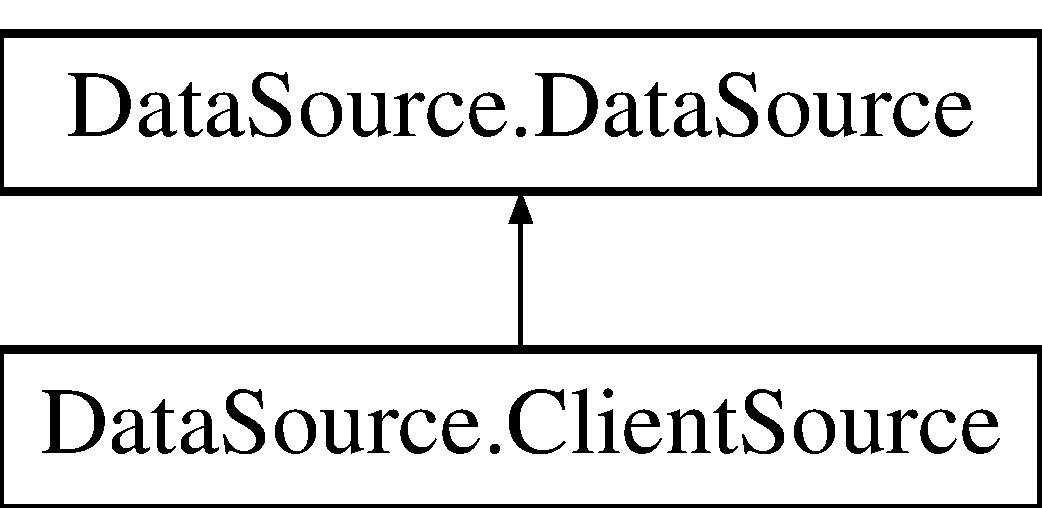
\includegraphics[height=2cm]{classDataSource_1_1ClientSource}
\end{center}
\end{figure}
\subsection*{Public Member Functions}
\begin{DoxyCompactItemize}
\item 
\hypertarget{classDataSource_1_1ClientSource_a24399ccfe037cd809da40142838feddc}{
def {\bfseries \_\-\_\-init\_\-\_\-}}
\label{classDataSource_1_1ClientSource_a24399ccfe037cd809da40142838feddc}

\item 
\hypertarget{classDataSource_1_1ClientSource_a1c021f74586206e3f81b7101a73ad506}{
def {\bfseries setJSON}}
\label{classDataSource_1_1ClientSource_a1c021f74586206e3f81b7101a73ad506}

\item 
\hypertarget{classDataSource_1_1ClientSource_a5b3cb19035b888e45cc22aa3a186b49d}{
def {\bfseries getData}}
\label{classDataSource_1_1ClientSource_a5b3cb19035b888e45cc22aa3a186b49d}

\end{DoxyCompactItemize}
\subsection*{Public Attributes}
\begin{DoxyCompactItemize}
\item 
\hypertarget{classDataSource_1_1ClientSource_ac39eb1a465b3588658ed953a8f896955}{
{\bfseries myJSON}}
\label{classDataSource_1_1ClientSource_ac39eb1a465b3588658ed953a8f896955}

\end{DoxyCompactItemize}


\subsection{Detailed Description}


Definition at line 125 of file DataSource.py.

The documentation for this class was generated from the following file:\begin{DoxyCompactItemize}
\item 
DataSource.py\end{DoxyCompactItemize}

\hypertarget{classDataHolder_1_1DataHolder}{
\section{DataHolder.DataHolder Class Reference}
\label{classDataHolder_1_1DataHolder}\index{DataHolder::DataHolder@{DataHolder::DataHolder}}
}
\subsection*{Public Member Functions}
\begin{DoxyCompactItemize}
\item 
def \hyperlink{classDataHolder_1_1DataHolder_a64f447d8ccac8ace2848733b9fb271fb}{\_\-\_\-init\_\-\_\-}
\item 
\hypertarget{classDataHolder_1_1DataHolder_a9030ee5d9b65208cde2c9d4dbcdfc071}{
def {\bfseries typeless\_\-array}}
\label{classDataHolder_1_1DataHolder_a9030ee5d9b65208cde2c9d4dbcdfc071}

\item 
\hypertarget{classDataHolder_1_1DataHolder_ad72b520efcaaecf3547c3fc048ae2368}{
def {\bfseries array}}
\label{classDataHolder_1_1DataHolder_ad72b520efcaaecf3547c3fc048ae2368}

\end{DoxyCompactItemize}
\subsection*{Public Attributes}
\begin{DoxyCompactItemize}
\item 
\hypertarget{classDataHolder_1_1DataHolder_a5d8a011784ef6bc9073eb224b7ad1125}{
{\bfseries format}}
\label{classDataHolder_1_1DataHolder_a5d8a011784ef6bc9073eb224b7ad1125}

\item 
\hypertarget{classDataHolder_1_1DataHolder_a85d4f33dd7f9ab88a0e5e7eb28b778a2}{
{\bfseries value}}
\label{classDataHolder_1_1DataHolder_a85d4f33dd7f9ab88a0e5e7eb28b778a2}

\item 
\hypertarget{classDataHolder_1_1DataHolder_a0c5d66f0a4ace660e2c327f5f786bee2}{
{\bfseries type}}
\label{classDataHolder_1_1DataHolder_a0c5d66f0a4ace660e2c327f5f786bee2}

\item 
\hypertarget{classDataHolder_1_1DataHolder_abe8269dcf9d02dd26c96e7615b2227d4}{
{\bfseries shape}}
\label{classDataHolder_1_1DataHolder_abe8269dcf9d02dd26c96e7615b2227d4}

\end{DoxyCompactItemize}


\subsection{Detailed Description}
\begin{DoxyVerb}A holder for passing data \end{DoxyVerb}
 

Definition at line 24 of file DataHolder.py.

\subsection{Member Function Documentation}
\hypertarget{classDataHolder_1_1DataHolder_a64f447d8ccac8ace2848733b9fb271fb}{
\index{DataHolder::DataHolder@{DataHolder::DataHolder}!\_\-\_\-init\_\-\_\-@{\_\-\_\-init\_\-\_\-}}
\index{\_\-\_\-init\_\-\_\-@{\_\-\_\-init\_\-\_\-}!DataHolder::DataHolder@{DataHolder::DataHolder}}
\subsubsection[{\_\-\_\-init\_\-\_\-}]{\setlength{\rightskip}{0pt plus 5cm}def DataHolder.DataHolder.\_\-\_\-init\_\-\_\- ( {\em self}, \/   {\em dFormat}, \/   {\em dValue}, \/   {\em dType}, \/   {\em dShape})}}
\label{classDataHolder_1_1DataHolder_a64f447d8ccac8ace2848733b9fb271fb}
\begin{DoxyVerb}Constructor \end{DoxyVerb}
 

Definition at line 26 of file DataHolder.py.

The documentation for this class was generated from the following file:\begin{DoxyCompactItemize}
\item 
DataHolder.py\end{DoxyCompactItemize}

\hypertarget{classDataSource_1_1DataSource}{
\section{DataSource.DataSource Class Reference}
\label{classDataSource_1_1DataSource}\index{DataSource::DataSource@{DataSource::DataSource}}
}
Inheritance diagram for DataSource.DataSource::\begin{figure}[H]
\begin{center}
\leavevmode
\includegraphics[height=1.55556cm]{classDataSource_1_1DataSource}
\end{center}
\end{figure}
\subsection*{Public Member Functions}
\begin{DoxyCompactItemize}
\item 
\hypertarget{classDataSource_1_1DataSource_a7ce54db00fe71393732da4cfc8d57473}{
def {\bfseries \_\-\_\-init\_\-\_\-}}
\label{classDataSource_1_1DataSource_a7ce54db00fe71393732da4cfc8d57473}

\item 
\hypertarget{classDataSource_1_1DataSource_abdd2f8aee9ac7903189095438b71615a}{
def {\bfseries getData}}
\label{classDataSource_1_1DataSource_abdd2f8aee9ac7903189095438b71615a}

\item 
\hypertarget{classDataSource_1_1DataSource_aff51edc77d07a3ba978438c6532e7788}{
def {\bfseries isValid}}
\label{classDataSource_1_1DataSource_aff51edc77d07a3ba978438c6532e7788}

\end{DoxyCompactItemize}
\subsection*{Public Attributes}
\begin{DoxyCompactItemize}
\item 
\hypertarget{classDataSource_1_1DataSource_a72186dfdb9c03491b8a5b2e1f0cc890a}{
{\bfseries strategy}}
\label{classDataSource_1_1DataSource_a72186dfdb9c03491b8a5b2e1f0cc890a}

\item 
\hypertarget{classDataSource_1_1DataSource_a14a4f8950ed084970fd8eb677bc59146}{
{\bfseries hostname}}
\label{classDataSource_1_1DataSource_a14a4f8950ed084970fd8eb677bc59146}

\item 
\hypertarget{classDataSource_1_1DataSource_a4db77848f62b1efc13d8e7e2b63ba627}{
{\bfseries port}}
\label{classDataSource_1_1DataSource_a4db77848f62b1efc13d8e7e2b63ba627}

\item 
\hypertarget{classDataSource_1_1DataSource_aa4461dfafb92f4aae91c005d27ae7f97}{
{\bfseries name}}
\label{classDataSource_1_1DataSource_aa4461dfafb92f4aae91c005d27ae7f97}

\end{DoxyCompactItemize}


\subsection{Detailed Description}


Definition at line 31 of file DataSource.py.

The documentation for this class was generated from the following file:\begin{DoxyCompactItemize}
\item 
DataSource.py\end{DoxyCompactItemize}

\hypertarget{classDataSource_1_1DataSourceFactory}{
\section{DataSource.DataSourceFactory Class Reference}
\label{classDataSource_1_1DataSourceFactory}\index{DataSource::DataSourceFactory@{DataSource::DataSourceFactory}}
}
Inheritance diagram for DataSource.DataSourceFactory::\begin{figure}[H]
\begin{center}
\leavevmode
\includegraphics[height=2cm]{classDataSource_1_1DataSourceFactory}
\end{center}
\end{figure}
\subsection*{Public Member Functions}
\begin{DoxyCompactItemize}
\item 
def \hyperlink{classDataSource_1_1DataSourceFactory_a9cfa373f259e0f9b21c9f1624fb7b517}{\_\-\_\-init\_\-\_\-}
\item 
\hypertarget{classDataSource_1_1DataSourceFactory_ac5399da5c150c5d766109dbd44670268}{
def {\bfseries createDSource}}
\label{classDataSource_1_1DataSourceFactory_ac5399da5c150c5d766109dbd44670268}

\end{DoxyCompactItemize}
\subsection*{Public Attributes}
\begin{DoxyCompactItemize}
\item 
\hypertarget{classDataSource_1_1DataSourceFactory_a95e0b3880f697952f85f9ec529e20396}{
{\bfseries sourceClass}}
\label{classDataSource_1_1DataSourceFactory_a95e0b3880f697952f85f9ec529e20396}

\end{DoxyCompactItemize}


\subsection{Detailed Description}


Definition at line 144 of file DataSource.py.

\subsection{Member Function Documentation}
\hypertarget{classDataSource_1_1DataSourceFactory_a9cfa373f259e0f9b21c9f1624fb7b517}{
\index{DataSource::DataSourceFactory@{DataSource::DataSourceFactory}!\_\-\_\-init\_\-\_\-@{\_\-\_\-init\_\-\_\-}}
\index{\_\-\_\-init\_\-\_\-@{\_\-\_\-init\_\-\_\-}!DataSource::DataSourceFactory@{DataSource::DataSourceFactory}}
\subsubsection[{\_\-\_\-init\_\-\_\-}]{\setlength{\rightskip}{0pt plus 5cm}def DataSource.DataSourceFactory.\_\-\_\-init\_\-\_\- ( {\em self}, \/   {\em name}, \/   {\em attrs}, \/   {\em last})}}
\label{classDataSource_1_1DataSourceFactory_a9cfa373f259e0f9b21c9f1624fb7b517}
\begin{DoxyVerb}Constructor \end{DoxyVerb}
 

Reimplemented from \hyperlink{classElement_1_1Element_a359371465b7c4d21611adec7e86c3b33}{Element.Element}.

Definition at line 145 of file DataSource.py.

The documentation for this class was generated from the following file:\begin{DoxyCompactItemize}
\item 
DataSource.py\end{DoxyCompactItemize}

\hypertarget{classDataSource_1_1DBaseSource}{
\section{DataSource.DBaseSource Class Reference}
\label{classDataSource_1_1DBaseSource}\index{DataSource::DBaseSource@{DataSource::DBaseSource}}
}
Inheritance diagram for DataSource.DBaseSource::\begin{figure}[H]
\begin{center}
\leavevmode
\includegraphics[height=2cm]{classDataSource_1_1DBaseSource}
\end{center}
\end{figure}
\subsection*{Public Member Functions}
\begin{DoxyCompactItemize}
\item 
\hypertarget{classDataSource_1_1DBaseSource_ab3704881ab5d142ce6a8b2951bd57bd6}{
def {\bfseries \_\-\_\-init\_\-\_\-}}
\label{classDataSource_1_1DBaseSource_ab3704881ab5d142ce6a8b2951bd57bd6}

\item 
\hypertarget{classDataSource_1_1DBaseSource_a0db468d8ece8092b352ad5a1745597e3}{
def {\bfseries getData}}
\label{classDataSource_1_1DBaseSource_a0db468d8ece8092b352ad5a1745597e3}

\end{DoxyCompactItemize}
\subsection*{Public Attributes}
\begin{DoxyCompactItemize}
\item 
\hypertarget{classDataSource_1_1DBaseSource_aee02199d2af33245fc9cc9741fb21f6e}{
{\bfseries query}}
\label{classDataSource_1_1DBaseSource_aee02199d2af33245fc9cc9741fb21f6e}

\item 
\hypertarget{classDataSource_1_1DBaseSource_ab0f88ad00efa0448a7f20b027c401a67}{
{\bfseries dbname}}
\label{classDataSource_1_1DBaseSource_ab0f88ad00efa0448a7f20b027c401a67}

\item 
\hypertarget{classDataSource_1_1DBaseSource_abeffcfbb2d7322f98a7ecbc0cf73db00}{
{\bfseries user}}
\label{classDataSource_1_1DBaseSource_abeffcfbb2d7322f98a7ecbc0cf73db00}

\item 
\hypertarget{classDataSource_1_1DBaseSource_ad9cb49eaabb02660c4840fc0d857becc}{
{\bfseries passwd}}
\label{classDataSource_1_1DBaseSource_ad9cb49eaabb02660c4840fc0d857becc}

\item 
\hypertarget{classDataSource_1_1DBaseSource_a98b07ec65665219f344450f9e8e94f74}{
{\bfseries mycnf}}
\label{classDataSource_1_1DBaseSource_a98b07ec65665219f344450f9e8e94f74}

\item 
\hypertarget{classDataSource_1_1DBaseSource_a06fa8663c0b689e1e657cbe52e73aabb}{
{\bfseries format}}
\label{classDataSource_1_1DBaseSource_a06fa8663c0b689e1e657cbe52e73aabb}

\end{DoxyCompactItemize}


\subsection{Detailed Description}


Definition at line 73 of file DataSource.py.

The documentation for this class was generated from the following file:\begin{DoxyCompactItemize}
\item 
DataSource.py\end{DoxyCompactItemize}

\hypertarget{classH5Elements_1_1EAttribute}{
\section{H5Elements.EAttribute Class Reference}
\label{classH5Elements_1_1EAttribute}\index{H5Elements::EAttribute@{H5Elements::EAttribute}}
}
Inheritance diagram for H5Elements.EAttribute::\begin{figure}[H]
\begin{center}
\leavevmode
\includegraphics[height=2cm]{classH5Elements_1_1EAttribute}
\end{center}
\end{figure}
\subsection*{Public Member Functions}
\begin{DoxyCompactItemize}
\item 
def \hyperlink{classH5Elements_1_1EAttribute_a42067c9a356fa17bbeb49de2acf9c438}{\_\-\_\-init\_\-\_\-}
\item 
\hypertarget{classH5Elements_1_1EAttribute_a0803bba087db250ff203d32f1facd69a}{
def {\bfseries store}}
\label{classH5Elements_1_1EAttribute_a0803bba087db250ff203d32f1facd69a}

\end{DoxyCompactItemize}


\subsection{Detailed Description}


Definition at line 344 of file H5Elements.py.

\subsection{Member Function Documentation}
\hypertarget{classH5Elements_1_1EAttribute_a42067c9a356fa17bbeb49de2acf9c438}{
\index{H5Elements::EAttribute@{H5Elements::EAttribute}!\_\-\_\-init\_\-\_\-@{\_\-\_\-init\_\-\_\-}}
\index{\_\-\_\-init\_\-\_\-@{\_\-\_\-init\_\-\_\-}!H5Elements::EAttribute@{H5Elements::EAttribute}}
\subsubsection[{\_\-\_\-init\_\-\_\-}]{\setlength{\rightskip}{0pt plus 5cm}def H5Elements.EAttribute.\_\-\_\-init\_\-\_\- ( {\em self}, \/   {\em name}, \/   {\em attrs}, \/   {\em last})}}
\label{classH5Elements_1_1EAttribute_a42067c9a356fa17bbeb49de2acf9c438}
\begin{DoxyVerb}Constructor \end{DoxyVerb}
 

Reimplemented from \hyperlink{classElement_1_1Element_a359371465b7c4d21611adec7e86c3b33}{Element.Element}.

Definition at line 345 of file H5Elements.py.

The documentation for this class was generated from the following file:\begin{DoxyCompactItemize}
\item 
H5Elements.py\end{DoxyCompactItemize}

\hypertarget{classH5Elements_1_1EDevice}{
\section{H5Elements.EDevice Class Reference}
\label{classH5Elements_1_1EDevice}\index{H5Elements::EDevice@{H5Elements::EDevice}}
}
Inheritance diagram for H5Elements.EDevice::\begin{figure}[H]
\begin{center}
\leavevmode
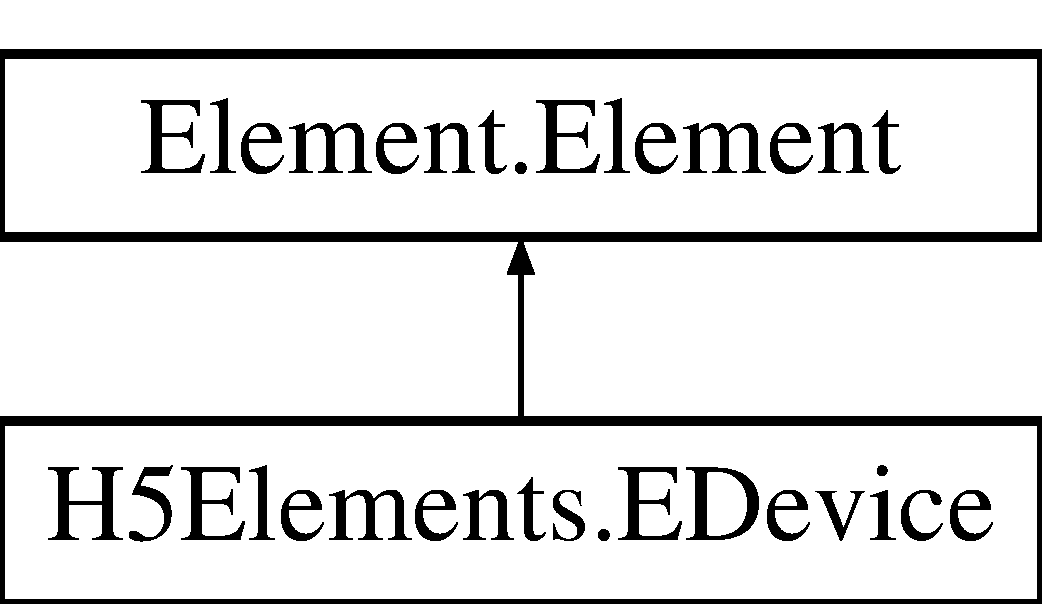
\includegraphics[height=2cm]{classH5Elements_1_1EDevice}
\end{center}
\end{figure}
\subsection*{Public Member Functions}
\begin{DoxyCompactItemize}
\item 
def \hyperlink{classH5Elements_1_1EDevice_a2ef0d670208549cb7eeafe75af802368}{\_\-\_\-init\_\-\_\-}
\end{DoxyCompactItemize}


\subsection{Detailed Description}


Definition at line 399 of file H5Elements.py.

\subsection{Member Function Documentation}
\hypertarget{classH5Elements_1_1EDevice_a2ef0d670208549cb7eeafe75af802368}{
\index{H5Elements::EDevice@{H5Elements::EDevice}!\_\-\_\-init\_\-\_\-@{\_\-\_\-init\_\-\_\-}}
\index{\_\-\_\-init\_\-\_\-@{\_\-\_\-init\_\-\_\-}!H5Elements::EDevice@{H5Elements::EDevice}}
\subsubsection[{\_\-\_\-init\_\-\_\-}]{\setlength{\rightskip}{0pt plus 5cm}def H5Elements.EDevice.\_\-\_\-init\_\-\_\- ( {\em self}, \/   {\em name}, \/   {\em attrs}, \/   {\em last})}}
\label{classH5Elements_1_1EDevice_a2ef0d670208549cb7eeafe75af802368}
\begin{DoxyVerb}Constructor \end{DoxyVerb}
 

Reimplemented from \hyperlink{classElement_1_1Element_a359371465b7c4d21611adec7e86c3b33}{Element.Element}.

Definition at line 400 of file H5Elements.py.

The documentation for this class was generated from the following file:\begin{DoxyCompactItemize}
\item 
H5Elements.py\end{DoxyCompactItemize}

\hypertarget{classH5Elements_1_1EDim}{
\section{H5Elements.EDim Class Reference}
\label{classH5Elements_1_1EDim}\index{H5Elements::EDim@{H5Elements::EDim}}
}
Inheritance diagram for H5Elements.EDim::\begin{figure}[H]
\begin{center}
\leavevmode
\includegraphics[height=2cm]{classH5Elements_1_1EDim}
\end{center}
\end{figure}
\subsection*{Public Member Functions}
\begin{DoxyCompactItemize}
\item 
def \hyperlink{classH5Elements_1_1EDim_ad40b269d818a529b5fbd09cab4d29d12}{\_\-\_\-init\_\-\_\-}
\end{DoxyCompactItemize}


\subsection{Detailed Description}


Definition at line 436 of file H5Elements.py.

\subsection{Member Function Documentation}
\hypertarget{classH5Elements_1_1EDim_ad40b269d818a529b5fbd09cab4d29d12}{
\index{H5Elements::EDim@{H5Elements::EDim}!\_\-\_\-init\_\-\_\-@{\_\-\_\-init\_\-\_\-}}
\index{\_\-\_\-init\_\-\_\-@{\_\-\_\-init\_\-\_\-}!H5Elements::EDim@{H5Elements::EDim}}
\subsubsection[{\_\-\_\-init\_\-\_\-}]{\setlength{\rightskip}{0pt plus 5cm}def H5Elements.EDim.\_\-\_\-init\_\-\_\- ( {\em self}, \/   {\em name}, \/   {\em attrs}, \/   {\em last})}}
\label{classH5Elements_1_1EDim_ad40b269d818a529b5fbd09cab4d29d12}
\begin{DoxyVerb}Constructor \end{DoxyVerb}
 

Reimplemented from \hyperlink{classElement_1_1Element_a359371465b7c4d21611adec7e86c3b33}{Element.Element}.

Definition at line 437 of file H5Elements.py.

The documentation for this class was generated from the following file:\begin{DoxyCompactItemize}
\item 
H5Elements.py\end{DoxyCompactItemize}

\hypertarget{classH5Elements_1_1EDimensions}{
\section{H5Elements.EDimensions Class Reference}
\label{classH5Elements_1_1EDimensions}\index{H5Elements::EDimensions@{H5Elements::EDimensions}}
}
Inheritance diagram for H5Elements.EDimensions::\begin{figure}[H]
\begin{center}
\leavevmode
\includegraphics[height=2cm]{classH5Elements_1_1EDimensions}
\end{center}
\end{figure}
\subsection*{Public Member Functions}
\begin{DoxyCompactItemize}
\item 
def \hyperlink{classH5Elements_1_1EDimensions_ac573211ddcc848f54103d9c68c903e6c}{\_\-\_\-init\_\-\_\-}
\end{DoxyCompactItemize}


\subsection{Detailed Description}


Definition at line 429 of file H5Elements.py.

\subsection{Member Function Documentation}
\hypertarget{classH5Elements_1_1EDimensions_ac573211ddcc848f54103d9c68c903e6c}{
\index{H5Elements::EDimensions@{H5Elements::EDimensions}!\_\-\_\-init\_\-\_\-@{\_\-\_\-init\_\-\_\-}}
\index{\_\-\_\-init\_\-\_\-@{\_\-\_\-init\_\-\_\-}!H5Elements::EDimensions@{H5Elements::EDimensions}}
\subsubsection[{\_\-\_\-init\_\-\_\-}]{\setlength{\rightskip}{0pt plus 5cm}def H5Elements.EDimensions.\_\-\_\-init\_\-\_\- ( {\em self}, \/   {\em name}, \/   {\em attrs}, \/   {\em last})}}
\label{classH5Elements_1_1EDimensions_ac573211ddcc848f54103d9c68c903e6c}
\begin{DoxyVerb}Constructor \end{DoxyVerb}
 

Reimplemented from \hyperlink{classElement_1_1Element_a359371465b7c4d21611adec7e86c3b33}{Element.Element}.

Definition at line 430 of file H5Elements.py.

The documentation for this class was generated from the following file:\begin{DoxyCompactItemize}
\item 
H5Elements.py\end{DoxyCompactItemize}

\hypertarget{classH5Elements_1_1EDoc}{
\section{H5Elements.EDoc Class Reference}
\label{classH5Elements_1_1EDoc}\index{H5Elements::EDoc@{H5Elements::EDoc}}
}
Inheritance diagram for H5Elements.EDoc::\begin{figure}[H]
\begin{center}
\leavevmode
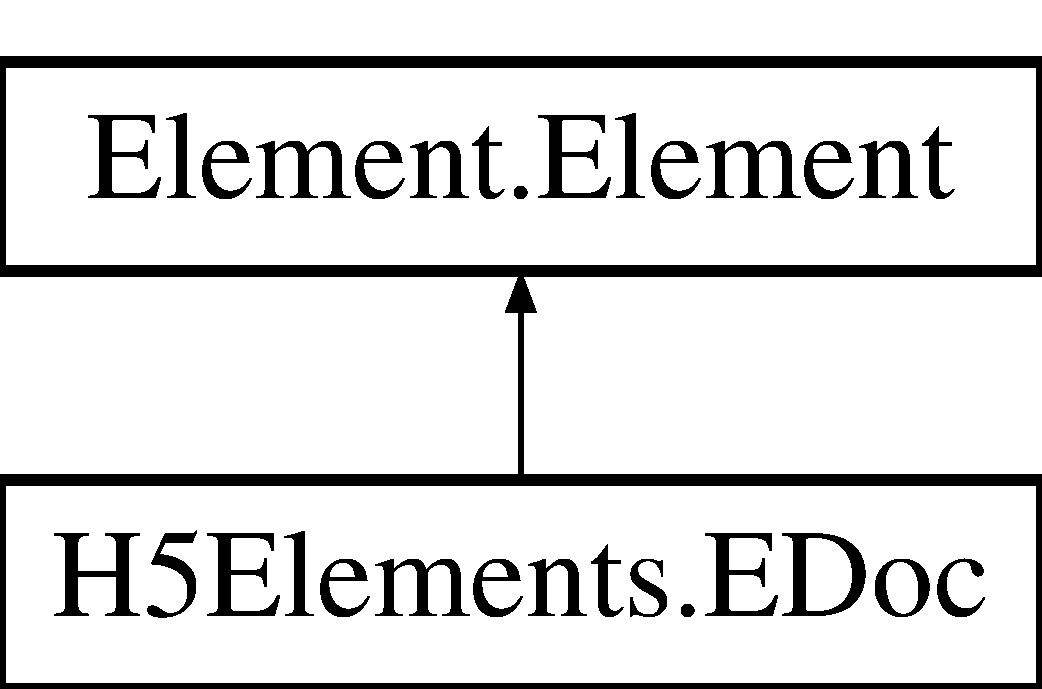
\includegraphics[height=2cm]{classH5Elements_1_1EDoc}
\end{center}
\end{figure}
\subsection*{Public Member Functions}
\begin{DoxyCompactItemize}
\item 
def \hyperlink{classH5Elements_1_1EDoc_a1680abdb0cd1799968e6661a70d1d341}{\_\-\_\-init\_\-\_\-}
\item 
\hypertarget{classH5Elements_1_1EDoc_a4ab92a516cf1b5f99995cc35ddcfbcba}{
def {\bfseries store}}
\label{classH5Elements_1_1EDoc_a4ab92a516cf1b5f99995cc35ddcfbcba}

\end{DoxyCompactItemize}


\subsection{Detailed Description}


Definition at line 371 of file H5Elements.py.

\subsection{Member Function Documentation}
\hypertarget{classH5Elements_1_1EDoc_a1680abdb0cd1799968e6661a70d1d341}{
\index{H5Elements::EDoc@{H5Elements::EDoc}!\_\-\_\-init\_\-\_\-@{\_\-\_\-init\_\-\_\-}}
\index{\_\-\_\-init\_\-\_\-@{\_\-\_\-init\_\-\_\-}!H5Elements::EDoc@{H5Elements::EDoc}}
\subsubsection[{\_\-\_\-init\_\-\_\-}]{\setlength{\rightskip}{0pt plus 5cm}def H5Elements.EDoc.\_\-\_\-init\_\-\_\- ( {\em self}, \/   {\em name}, \/   {\em attrs}, \/   {\em last})}}
\label{classH5Elements_1_1EDoc_a1680abdb0cd1799968e6661a70d1d341}
\begin{DoxyVerb}Constructor \end{DoxyVerb}
 

Reimplemented from \hyperlink{classElement_1_1Element_a359371465b7c4d21611adec7e86c3b33}{Element.Element}.

Definition at line 372 of file H5Elements.py.

The documentation for this class was generated from the following file:\begin{DoxyCompactItemize}
\item 
H5Elements.py\end{DoxyCompactItemize}

\hypertarget{classH5Elements_1_1EDoor}{
\section{H5Elements.EDoor Class Reference}
\label{classH5Elements_1_1EDoor}\index{H5Elements::EDoor@{H5Elements::EDoor}}
}
Inheritance diagram for H5Elements.EDoor::\begin{figure}[H]
\begin{center}
\leavevmode
\includegraphics[height=2cm]{classH5Elements_1_1EDoor}
\end{center}
\end{figure}
\subsection*{Public Member Functions}
\begin{DoxyCompactItemize}
\item 
def \hyperlink{classH5Elements_1_1EDoor_ae4bda86f18b9555bc435883e109415a9}{\_\-\_\-init\_\-\_\-}
\end{DoxyCompactItemize}


\subsection{Detailed Description}


Definition at line 405 of file H5Elements.py.

\subsection{Member Function Documentation}
\hypertarget{classH5Elements_1_1EDoor_ae4bda86f18b9555bc435883e109415a9}{
\index{H5Elements::EDoor@{H5Elements::EDoor}!\_\-\_\-init\_\-\_\-@{\_\-\_\-init\_\-\_\-}}
\index{\_\-\_\-init\_\-\_\-@{\_\-\_\-init\_\-\_\-}!H5Elements::EDoor@{H5Elements::EDoor}}
\subsubsection[{\_\-\_\-init\_\-\_\-}]{\setlength{\rightskip}{0pt plus 5cm}def H5Elements.EDoor.\_\-\_\-init\_\-\_\- ( {\em self}, \/   {\em name}, \/   {\em attrs}, \/   {\em last})}}
\label{classH5Elements_1_1EDoor_ae4bda86f18b9555bc435883e109415a9}
\begin{DoxyVerb}Constructor \end{DoxyVerb}
 

Reimplemented from \hyperlink{classElement_1_1Element_a359371465b7c4d21611adec7e86c3b33}{Element.Element}.

Definition at line 406 of file H5Elements.py.

The documentation for this class was generated from the following file:\begin{DoxyCompactItemize}
\item 
H5Elements.py\end{DoxyCompactItemize}

\hypertarget{classH5Elements_1_1EField}{
\section{H5Elements.EField Class Reference}
\label{classH5Elements_1_1EField}\index{H5Elements::EField@{H5Elements::EField}}
}
Inheritance diagram for H5Elements.EField::\begin{figure}[H]
\begin{center}
\leavevmode
\includegraphics[height=3cm]{classH5Elements_1_1EField}
\end{center}
\end{figure}
\subsection*{Public Member Functions}
\begin{DoxyCompactItemize}
\item 
def \hyperlink{classH5Elements_1_1EField_ad58a5277143c1a17c5e004c92081d937}{\_\-\_\-init\_\-\_\-}
\item 
\hypertarget{classH5Elements_1_1EField_a840c5d5bebc6d08587c2d8a06dbbe3d2}{
def {\bfseries store}}
\label{classH5Elements_1_1EField_a840c5d5bebc6d08587c2d8a06dbbe3d2}

\item 
\hypertarget{classH5Elements_1_1EField_a49582f2fbeefde265a26e5f679a47f9e}{
def {\bfseries run}}
\label{classH5Elements_1_1EField_a49582f2fbeefde265a26e5f679a47f9e}

\end{DoxyCompactItemize}
\subsection*{Public Attributes}
\begin{DoxyCompactItemize}
\item 
\hypertarget{classH5Elements_1_1EField_a20fcb945f9ef6edef2c9f985130b1027}{
{\bfseries rank}}
\label{classH5Elements_1_1EField_a20fcb945f9ef6edef2c9f985130b1027}

\item 
\hypertarget{classH5Elements_1_1EField_a0eb574a560fd8be9ff14e3672fae3d7d}{
{\bfseries lengths}}
\label{classH5Elements_1_1EField_a0eb574a560fd8be9ff14e3672fae3d7d}

\item 
\hypertarget{classH5Elements_1_1EField_a4279511bf17bbc59fbf1fe19408a98e8}{
{\bfseries tpAttrs}}
\label{classH5Elements_1_1EField_a4279511bf17bbc59fbf1fe19408a98e8}

\item 
\hypertarget{classH5Elements_1_1EField_a5f0837583c5bf72ca38465ad218305d1}{
{\bfseries extraD}}
\label{classH5Elements_1_1EField_a5f0837583c5bf72ca38465ad218305d1}

\item 
\hypertarget{classH5Elements_1_1EField_ae8797dcd699ca34be6e5e20d73559250}{
\hyperlink{classH5Elements_1_1EField_ae8797dcd699ca34be6e5e20d73559250}{fObject}}
\label{classH5Elements_1_1EField_ae8797dcd699ca34be6e5e20d73559250}

\begin{DoxyCompactList}\small\item\em Stored tag object. \item\end{DoxyCompactList}\end{DoxyCompactItemize}


\subsection{Detailed Description}


Definition at line 127 of file H5Elements.py.

\subsection{Member Function Documentation}
\hypertarget{classH5Elements_1_1EField_ad58a5277143c1a17c5e004c92081d937}{
\index{H5Elements::EField@{H5Elements::EField}!\_\-\_\-init\_\-\_\-@{\_\-\_\-init\_\-\_\-}}
\index{\_\-\_\-init\_\-\_\-@{\_\-\_\-init\_\-\_\-}!H5Elements::EField@{H5Elements::EField}}
\subsubsection[{\_\-\_\-init\_\-\_\-}]{\setlength{\rightskip}{0pt plus 5cm}def H5Elements.EField.\_\-\_\-init\_\-\_\- ( {\em self}, \/   {\em name}, \/   {\em attrs}, \/   {\em last})}}
\label{classH5Elements_1_1EField_ad58a5277143c1a17c5e004c92081d937}
\begin{DoxyVerb}Constructor \end{DoxyVerb}
 

Reimplemented from \hyperlink{classElement_1_1Element_a359371465b7c4d21611adec7e86c3b33}{Element.Element}.

Definition at line 128 of file H5Elements.py.

The documentation for this class was generated from the following file:\begin{DoxyCompactItemize}
\item 
H5Elements.py\end{DoxyCompactItemize}

\hypertarget{classH5Elements_1_1EFile}{
\section{H5Elements.EFile Class Reference}
\label{classH5Elements_1_1EFile}\index{H5Elements::EFile@{H5Elements::EFile}}
}
Inheritance diagram for H5Elements.EFile::\begin{figure}[H]
\begin{center}
\leavevmode
\includegraphics[height=3cm]{classH5Elements_1_1EFile}
\end{center}
\end{figure}
\subsection*{Public Member Functions}
\begin{DoxyCompactItemize}
\item 
def \hyperlink{classH5Elements_1_1EFile_a8583b07993d4f52b537bb202bdb39863}{\_\-\_\-init\_\-\_\-}
\end{DoxyCompactItemize}


\subsection{Detailed Description}


Definition at line 365 of file H5Elements.py.

\subsection{Member Function Documentation}
\hypertarget{classH5Elements_1_1EFile_a8583b07993d4f52b537bb202bdb39863}{
\index{H5Elements::EFile@{H5Elements::EFile}!\_\-\_\-init\_\-\_\-@{\_\-\_\-init\_\-\_\-}}
\index{\_\-\_\-init\_\-\_\-@{\_\-\_\-init\_\-\_\-}!H5Elements::EFile@{H5Elements::EFile}}
\subsubsection[{\_\-\_\-init\_\-\_\-}]{\setlength{\rightskip}{0pt plus 5cm}def H5Elements.EFile.\_\-\_\-init\_\-\_\- ( {\em self}, \/   {\em name}, \/   {\em attrs}, \/   {\em last}, \/   {\em obj})}}
\label{classH5Elements_1_1EFile_a8583b07993d4f52b537bb202bdb39863}
\begin{DoxyVerb}Constructor \end{DoxyVerb}
 

Reimplemented from \hyperlink{classH5Elements_1_1FElement_ac013d152339bec50771f059a62e764c7}{H5Elements.FElement}.

Definition at line 366 of file H5Elements.py.

The documentation for this class was generated from the following file:\begin{DoxyCompactItemize}
\item 
H5Elements.py\end{DoxyCompactItemize}

\hypertarget{classH5Elements_1_1EGroup}{
\section{H5Elements.EGroup Class Reference}
\label{classH5Elements_1_1EGroup}\index{H5Elements::EGroup@{H5Elements::EGroup}}
}
Inheritance diagram for H5Elements.EGroup::\begin{figure}[H]
\begin{center}
\leavevmode
\includegraphics[height=3cm]{classH5Elements_1_1EGroup}
\end{center}
\end{figure}
\subsection*{Public Member Functions}
\begin{DoxyCompactItemize}
\item 
def \hyperlink{classH5Elements_1_1EGroup_a3ab898c36d1fa91a226417a3296a651b}{\_\-\_\-init\_\-\_\-}
\item 
\hypertarget{classH5Elements_1_1EGroup_a16ec0be870d3751c0af90b2fb64e34cc}{
def {\bfseries store}}
\label{classH5Elements_1_1EGroup_a16ec0be870d3751c0af90b2fb64e34cc}

\item 
\hypertarget{classH5Elements_1_1EGroup_abccdc92a4b4de689590502b11a0820af}{
def {\bfseries fetchName}}
\label{classH5Elements_1_1EGroup_abccdc92a4b4de689590502b11a0820af}

\end{DoxyCompactItemize}
\subsection*{Public Attributes}
\begin{DoxyCompactItemize}
\item 
\hypertarget{classH5Elements_1_1EGroup_af0bee9c867e8b439a291ab2f09f2516e}{
{\bfseries tpAttrs}}
\label{classH5Elements_1_1EGroup_af0bee9c867e8b439a291ab2f09f2516e}

\item 
\hypertarget{classH5Elements_1_1EGroup_aeb9bf60e89f45e2df375c9e5081e736d}{
\hyperlink{classH5Elements_1_1EGroup_aeb9bf60e89f45e2df375c9e5081e736d}{fObject}}
\label{classH5Elements_1_1EGroup_aeb9bf60e89f45e2df375c9e5081e736d}

\begin{DoxyCompactList}\small\item\em Stored tag object. \item\end{DoxyCompactList}\end{DoxyCompactItemize}


\subsection{Detailed Description}


Definition at line 260 of file H5Elements.py.

\subsection{Member Function Documentation}
\hypertarget{classH5Elements_1_1EGroup_a3ab898c36d1fa91a226417a3296a651b}{
\index{H5Elements::EGroup@{H5Elements::EGroup}!\_\-\_\-init\_\-\_\-@{\_\-\_\-init\_\-\_\-}}
\index{\_\-\_\-init\_\-\_\-@{\_\-\_\-init\_\-\_\-}!H5Elements::EGroup@{H5Elements::EGroup}}
\subsubsection[{\_\-\_\-init\_\-\_\-}]{\setlength{\rightskip}{0pt plus 5cm}def H5Elements.EGroup.\_\-\_\-init\_\-\_\- ( {\em self}, \/   {\em name}, \/   {\em attrs}, \/   {\em last})}}
\label{classH5Elements_1_1EGroup_a3ab898c36d1fa91a226417a3296a651b}
\begin{DoxyVerb}Constructor \end{DoxyVerb}
 

Reimplemented from \hyperlink{classElement_1_1Element_a359371465b7c4d21611adec7e86c3b33}{Element.Element}.

Definition at line 261 of file H5Elements.py.

The documentation for this class was generated from the following file:\begin{DoxyCompactItemize}
\item 
H5Elements.py\end{DoxyCompactItemize}

\hypertarget{classElement_1_1Element}{
\section{Element.Element Class Reference}
\label{classElement_1_1Element}\index{Element::Element@{Element::Element}}
}
Inheritance diagram for Element.Element::\begin{figure}[H]
\begin{center}
\leavevmode
\includegraphics[height=12cm]{classElement_1_1Element}
\end{center}
\end{figure}
\subsection*{Public Member Functions}
\begin{DoxyCompactItemize}
\item 
def \hyperlink{classElement_1_1Element_a359371465b7c4d21611adec7e86c3b33}{\_\-\_\-init\_\-\_\-}
\item 
\hypertarget{classElement_1_1Element_a44825d29e1f59b7c8f0ebe7710df530e}{
def {\bfseries lastObject}}
\label{classElement_1_1Element_a44825d29e1f59b7c8f0ebe7710df530e}

\item 
\hypertarget{classElement_1_1Element_a5e75dc810e645f7f2411d10e7b1db0f3}{
def {\bfseries beforeLast}}
\label{classElement_1_1Element_a5e75dc810e645f7f2411d10e7b1db0f3}

\item 
\hypertarget{classElement_1_1Element_a382e33855f5875d4d56af8249ceb2cff}{
def {\bfseries store}}
\label{classElement_1_1Element_a382e33855f5875d4d56af8249ceb2cff}

\end{DoxyCompactItemize}
\subsection*{Public Attributes}
\begin{DoxyCompactItemize}
\item 
\hypertarget{classElement_1_1Element_a4729b44d681267785171f594798a4b18}{
\hyperlink{classElement_1_1Element_a4729b44d681267785171f594798a4b18}{tName}}
\label{classElement_1_1Element_a4729b44d681267785171f594798a4b18}

\begin{DoxyCompactList}\small\item\em Stored tag name. \item\end{DoxyCompactList}\item 
\hypertarget{classElement_1_1Element_abe80105d47b38b08c866d66cba5e361c}{
{\bfseries tAttrs}}
\label{classElement_1_1Element_abe80105d47b38b08c866d66cba5e361c}

\item 
\hypertarget{classElement_1_1Element_a44f8f4eb9a4584267749534b65d50e49}{
\hyperlink{classElement_1_1Element_a44f8f4eb9a4584267749534b65d50e49}{doc}}
\label{classElement_1_1Element_a44f8f4eb9a4584267749534b65d50e49}

\begin{DoxyCompactList}\small\item\em Stored tag content. \item\end{DoxyCompactList}\item 
\hypertarget{classElement_1_1Element_af672c1031cebcdfbe6f1aed263eab0fb}{
{\bfseries content}}
\label{classElement_1_1Element_af672c1031cebcdfbe6f1aed263eab0fb}

\item 
\hypertarget{classElement_1_1Element_a61228f20b35d5eda65d64cb1250c12f2}{
{\bfseries last}}
\label{classElement_1_1Element_a61228f20b35d5eda65d64cb1250c12f2}

\end{DoxyCompactItemize}


\subsection{Detailed Description}
\begin{DoxyVerb}A tag element stored on our stack  \end{DoxyVerb}
 

Definition at line 23 of file Element.py.

\subsection{Member Function Documentation}
\hypertarget{classElement_1_1Element_a359371465b7c4d21611adec7e86c3b33}{
\index{Element::Element@{Element::Element}!\_\-\_\-init\_\-\_\-@{\_\-\_\-init\_\-\_\-}}
\index{\_\-\_\-init\_\-\_\-@{\_\-\_\-init\_\-\_\-}!Element::Element@{Element::Element}}
\subsubsection[{\_\-\_\-init\_\-\_\-}]{\setlength{\rightskip}{0pt plus 5cm}def Element.Element.\_\-\_\-init\_\-\_\- ( {\em self}, \/   {\em name}, \/   {\em attrs}, \/   {\em last} = {\ttfamily None})}}
\label{classElement_1_1Element_a359371465b7c4d21611adec7e86c3b33}
\begin{DoxyVerb}Constructor \end{DoxyVerb}
 

Reimplemented in \hyperlink{classDataSource_1_1DataSourceFactory_a9cfa373f259e0f9b21c9f1624fb7b517}{DataSource.DataSourceFactory}, \hyperlink{classH5Elements_1_1EField_ad58a5277143c1a17c5e004c92081d937}{H5Elements.EField}, \hyperlink{classH5Elements_1_1EGroup_a3ab898c36d1fa91a226417a3296a651b}{H5Elements.EGroup}, \hyperlink{classH5Elements_1_1ELink_a15f6a1e9476b5ef916b597243a79b0e8}{H5Elements.ELink}, \hyperlink{classH5Elements_1_1EAttribute_a42067c9a356fa17bbeb49de2acf9c438}{H5Elements.EAttribute}, \hyperlink{classH5Elements_1_1EDoc_a1680abdb0cd1799968e6661a70d1d341}{H5Elements.EDoc}, \hyperlink{classH5Elements_1_1ESymbol_ae29345c630720f8c56b66c6ab74c39be}{H5Elements.ESymbol}, \hyperlink{classH5Elements_1_1ERecord_a11c91d973c319626d283c13a2679140b}{H5Elements.ERecord}, \hyperlink{classH5Elements_1_1EDevice_a2ef0d670208549cb7eeafe75af802368}{H5Elements.EDevice}, \hyperlink{classH5Elements_1_1EDoor_ae4bda86f18b9555bc435883e109415a9}{H5Elements.EDoor}, \hyperlink{classH5Elements_1_1EQuery_a4762ac1d81b6253845dc4a179880ffd9}{H5Elements.EQuery}, \hyperlink{classH5Elements_1_1EDimensions_ac573211ddcc848f54103d9c68c903e6c}{H5Elements.EDimensions}, and \hyperlink{classH5Elements_1_1EDim_ad40b269d818a529b5fbd09cab4d29d12}{H5Elements.EDim}.

Definition at line 25 of file Element.py.

The documentation for this class was generated from the following file:\begin{DoxyCompactItemize}
\item 
Element.py\end{DoxyCompactItemize}

\hypertarget{classElementThread_1_1ElementThread}{
\section{ElementThread.ElementThread Class Reference}
\label{classElementThread_1_1ElementThread}\index{ElementThread::ElementThread@{ElementThread::ElementThread}}
}
\subsection*{Public Member Functions}
\begin{DoxyCompactItemize}
\item 
\hypertarget{classElementThread_1_1ElementThread_a5187bb7f94a5270c8f58bae314304aa0}{
def {\bfseries \_\-\_\-init\_\-\_\-}}
\label{classElementThread_1_1ElementThread_a5187bb7f94a5270c8f58bae314304aa0}

\item 
\hypertarget{classElementThread_1_1ElementThread_a6cb9235cd455f78840240d73408e52d8}{
def {\bfseries run}}
\label{classElementThread_1_1ElementThread_a6cb9235cd455f78840240d73408e52d8}

\end{DoxyCompactItemize}
\subsection*{Public Attributes}
\begin{DoxyCompactItemize}
\item 
\hypertarget{classElementThread_1_1ElementThread_a48717674c63b31a3e7a9c3f7a524f3a2}{
{\bfseries elem}}
\label{classElementThread_1_1ElementThread_a48717674c63b31a3e7a9c3f7a524f3a2}

\end{DoxyCompactItemize}


\subsection{Detailed Description}
\begin{DoxyVerb}Pool of Threads \end{DoxyVerb}
 

Definition at line 24 of file ElementThread.py.

The documentation for this class was generated from the following file:\begin{DoxyCompactItemize}
\item 
ElementThread.py\end{DoxyCompactItemize}

\hypertarget{classH5Elements_1_1ELink}{
\section{H5Elements.ELink Class Reference}
\label{classH5Elements_1_1ELink}\index{H5Elements::ELink@{H5Elements::ELink}}
}
Inheritance diagram for H5Elements.ELink::\begin{figure}[H]
\begin{center}
\leavevmode
\includegraphics[height=3cm]{classH5Elements_1_1ELink}
\end{center}
\end{figure}
\subsection*{Public Member Functions}
\begin{DoxyCompactItemize}
\item 
def \hyperlink{classH5Elements_1_1ELink_a15f6a1e9476b5ef916b597243a79b0e8}{\_\-\_\-init\_\-\_\-}
\item 
def \hyperlink{classH5Elements_1_1ELink_acc66ee4d29d63fd921d96974e45413fc}{typesToNames}
\item 
\hypertarget{classH5Elements_1_1ELink_ad55d058f16bea9ebc8c2a746bf67689a}{
def {\bfseries createLink}}
\label{classH5Elements_1_1ELink_ad55d058f16bea9ebc8c2a746bf67689a}

\end{DoxyCompactItemize}
\subsection*{Public Attributes}
\begin{DoxyCompactItemize}
\item 
\hypertarget{classH5Elements_1_1ELink_a3b71ab0736b0ce0c69d59f91cf6ee107}{
\hyperlink{classH5Elements_1_1ELink_a3b71ab0736b0ce0c69d59f91cf6ee107}{fObject}}
\label{classH5Elements_1_1ELink_a3b71ab0736b0ce0c69d59f91cf6ee107}

\begin{DoxyCompactList}\small\item\em Stored tag object. \item\end{DoxyCompactList}\end{DoxyCompactItemize}


\subsection{Detailed Description}


Definition at line 302 of file H5Elements.py.

\subsection{Member Function Documentation}
\hypertarget{classH5Elements_1_1ELink_a15f6a1e9476b5ef916b597243a79b0e8}{
\index{H5Elements::ELink@{H5Elements::ELink}!\_\-\_\-init\_\-\_\-@{\_\-\_\-init\_\-\_\-}}
\index{\_\-\_\-init\_\-\_\-@{\_\-\_\-init\_\-\_\-}!H5Elements::ELink@{H5Elements::ELink}}
\subsubsection[{\_\-\_\-init\_\-\_\-}]{\setlength{\rightskip}{0pt plus 5cm}def H5Elements.ELink.\_\-\_\-init\_\-\_\- ( {\em self}, \/   {\em name}, \/   {\em attrs}, \/   {\em last})}}
\label{classH5Elements_1_1ELink_a15f6a1e9476b5ef916b597243a79b0e8}
\begin{DoxyVerb}Constructor \end{DoxyVerb}
 

Reimplemented from \hyperlink{classElement_1_1Element_a359371465b7c4d21611adec7e86c3b33}{Element.Element}.

Definition at line 303 of file H5Elements.py.\hypertarget{classH5Elements_1_1ELink_acc66ee4d29d63fd921d96974e45413fc}{
\index{H5Elements::ELink@{H5Elements::ELink}!typesToNames@{typesToNames}}
\index{typesToNames@{typesToNames}!H5Elements::ELink@{H5Elements::ELink}}
\subsubsection[{typesToNames}]{\setlength{\rightskip}{0pt plus 5cm}def H5Elements.ELink.typesToNames ( {\em self}, \/   {\em text}, \/   {\em groupTypes})}}
\label{classH5Elements_1_1ELink_acc66ee4d29d63fd921d96974e45413fc}
\begin{DoxyVerb}converts NXclass types to names in a path string\end{DoxyVerb}
 

Definition at line 307 of file H5Elements.py.

The documentation for this class was generated from the following file:\begin{DoxyCompactItemize}
\item 
H5Elements.py\end{DoxyCompactItemize}

\hypertarget{classH5Elements_1_1EQuery}{
\section{H5Elements.EQuery Class Reference}
\label{classH5Elements_1_1EQuery}\index{H5Elements::EQuery@{H5Elements::EQuery}}
}
Inheritance diagram for H5Elements.EQuery::\begin{figure}[H]
\begin{center}
\leavevmode
\includegraphics[height=2cm]{classH5Elements_1_1EQuery}
\end{center}
\end{figure}
\subsection*{Public Member Functions}
\begin{DoxyCompactItemize}
\item 
def \hyperlink{classH5Elements_1_1EQuery_a4762ac1d81b6253845dc4a179880ffd9}{\_\-\_\-init\_\-\_\-}
\item 
\hypertarget{classH5Elements_1_1EQuery_a42591031918d8de7cee72a1f66f5da9e}{
def {\bfseries store}}
\label{classH5Elements_1_1EQuery_a42591031918d8de7cee72a1f66f5da9e}

\end{DoxyCompactItemize}


\subsection{Detailed Description}


Definition at line 412 of file H5Elements.py.

\subsection{Member Function Documentation}
\hypertarget{classH5Elements_1_1EQuery_a4762ac1d81b6253845dc4a179880ffd9}{
\index{H5Elements::EQuery@{H5Elements::EQuery}!\_\-\_\-init\_\-\_\-@{\_\-\_\-init\_\-\_\-}}
\index{\_\-\_\-init\_\-\_\-@{\_\-\_\-init\_\-\_\-}!H5Elements::EQuery@{H5Elements::EQuery}}
\subsubsection[{\_\-\_\-init\_\-\_\-}]{\setlength{\rightskip}{0pt plus 5cm}def H5Elements.EQuery.\_\-\_\-init\_\-\_\- ( {\em self}, \/   {\em name}, \/   {\em attrs}, \/   {\em last})}}
\label{classH5Elements_1_1EQuery_a4762ac1d81b6253845dc4a179880ffd9}
\begin{DoxyVerb}Constructor \end{DoxyVerb}
 

Reimplemented from \hyperlink{classElement_1_1Element_a359371465b7c4d21611adec7e86c3b33}{Element.Element}.

Definition at line 413 of file H5Elements.py.

The documentation for this class was generated from the following file:\begin{DoxyCompactItemize}
\item 
H5Elements.py\end{DoxyCompactItemize}

\hypertarget{classH5Elements_1_1ERecord}{
\section{H5Elements.ERecord Class Reference}
\label{classH5Elements_1_1ERecord}\index{H5Elements::ERecord@{H5Elements::ERecord}}
}
Inheritance diagram for H5Elements.ERecord::\begin{figure}[H]
\begin{center}
\leavevmode
\includegraphics[height=2cm]{classH5Elements_1_1ERecord}
\end{center}
\end{figure}
\subsection*{Public Member Functions}
\begin{DoxyCompactItemize}
\item 
def \hyperlink{classH5Elements_1_1ERecord_a11c91d973c319626d283c13a2679140b}{\_\-\_\-init\_\-\_\-}
\end{DoxyCompactItemize}


\subsection{Detailed Description}


Definition at line 390 of file H5Elements.py.

\subsection{Member Function Documentation}
\hypertarget{classH5Elements_1_1ERecord_a11c91d973c319626d283c13a2679140b}{
\index{H5Elements::ERecord@{H5Elements::ERecord}!\_\-\_\-init\_\-\_\-@{\_\-\_\-init\_\-\_\-}}
\index{\_\-\_\-init\_\-\_\-@{\_\-\_\-init\_\-\_\-}!H5Elements::ERecord@{H5Elements::ERecord}}
\subsubsection[{\_\-\_\-init\_\-\_\-}]{\setlength{\rightskip}{0pt plus 5cm}def H5Elements.ERecord.\_\-\_\-init\_\-\_\- ( {\em self}, \/   {\em name}, \/   {\em attrs}, \/   {\em last})}}
\label{classH5Elements_1_1ERecord_a11c91d973c319626d283c13a2679140b}
\begin{DoxyVerb}Constructor \end{DoxyVerb}
 

Reimplemented from \hyperlink{classElement_1_1Element_a359371465b7c4d21611adec7e86c3b33}{Element.Element}.

Definition at line 391 of file H5Elements.py.

The documentation for this class was generated from the following file:\begin{DoxyCompactItemize}
\item 
H5Elements.py\end{DoxyCompactItemize}

\hypertarget{classH5Elements_1_1ESymbol}{
\section{H5Elements.ESymbol Class Reference}
\label{classH5Elements_1_1ESymbol}\index{H5Elements::ESymbol@{H5Elements::ESymbol}}
}
Inheritance diagram for H5Elements.ESymbol::\begin{figure}[H]
\begin{center}
\leavevmode
\includegraphics[height=2cm]{classH5Elements_1_1ESymbol}
\end{center}
\end{figure}
\subsection*{Public Member Functions}
\begin{DoxyCompactItemize}
\item 
def \hyperlink{classH5Elements_1_1ESymbol_ae29345c630720f8c56b66c6ab74c39be}{\_\-\_\-init\_\-\_\-}
\item 
\hypertarget{classH5Elements_1_1ESymbol_aef5a885ba867f51e723db359e41f6280}{
def {\bfseries store}}
\label{classH5Elements_1_1ESymbol_aef5a885ba867f51e723db359e41f6280}

\end{DoxyCompactItemize}
\subsection*{Public Attributes}
\begin{DoxyCompactItemize}
\item 
\hypertarget{classH5Elements_1_1ESymbol_aa12375c96285f20a725ff953a6d017b8}{
{\bfseries symbols}}
\label{classH5Elements_1_1ESymbol_aa12375c96285f20a725ff953a6d017b8}

\end{DoxyCompactItemize}


\subsection{Detailed Description}


Definition at line 379 of file H5Elements.py.

\subsection{Member Function Documentation}
\hypertarget{classH5Elements_1_1ESymbol_ae29345c630720f8c56b66c6ab74c39be}{
\index{H5Elements::ESymbol@{H5Elements::ESymbol}!\_\-\_\-init\_\-\_\-@{\_\-\_\-init\_\-\_\-}}
\index{\_\-\_\-init\_\-\_\-@{\_\-\_\-init\_\-\_\-}!H5Elements::ESymbol@{H5Elements::ESymbol}}
\subsubsection[{\_\-\_\-init\_\-\_\-}]{\setlength{\rightskip}{0pt plus 5cm}def H5Elements.ESymbol.\_\-\_\-init\_\-\_\- ( {\em self}, \/   {\em name}, \/   {\em attrs}, \/   {\em last})}}
\label{classH5Elements_1_1ESymbol_ae29345c630720f8c56b66c6ab74c39be}
\begin{DoxyVerb}Constructor \end{DoxyVerb}
 

Reimplemented from \hyperlink{classElement_1_1Element_a359371465b7c4d21611adec7e86c3b33}{Element.Element}.

Definition at line 380 of file H5Elements.py.

The documentation for this class was generated from the following file:\begin{DoxyCompactItemize}
\item 
H5Elements.py\end{DoxyCompactItemize}

\hypertarget{classH5Elements_1_1FElement}{
\section{H5Elements.FElement Class Reference}
\label{classH5Elements_1_1FElement}\index{H5Elements::FElement@{H5Elements::FElement}}
}
Inheritance diagram for H5Elements.FElement::\begin{figure}[H]
\begin{center}
\leavevmode
\includegraphics[height=2.95775cm]{classH5Elements_1_1FElement}
\end{center}
\end{figure}
\subsection*{Public Member Functions}
\begin{DoxyCompactItemize}
\item 
def \hyperlink{classH5Elements_1_1FElement_ac013d152339bec50771f059a62e764c7}{\_\-\_\-init\_\-\_\-}
\item 
\hypertarget{classH5Elements_1_1FElement_ab857523cc7673e38615eca1c808d6663}{
def {\bfseries run}}
\label{classH5Elements_1_1FElement_ab857523cc7673e38615eca1c808d6663}

\end{DoxyCompactItemize}
\subsection*{Public Attributes}
\begin{DoxyCompactItemize}
\item 
\hypertarget{classH5Elements_1_1FElement_a09a6294d06d1bdaf337218bc9db31309}{
\hyperlink{classH5Elements_1_1FElement_a09a6294d06d1bdaf337218bc9db31309}{fObject}}
\label{classH5Elements_1_1FElement_a09a6294d06d1bdaf337218bc9db31309}

\begin{DoxyCompactList}\small\item\em Stored tag object. \item\end{DoxyCompactList}\item 
\hypertarget{classH5Elements_1_1FElement_afa877c4dd573134f9483a9a35deedda7}{
{\bfseries source}}
\label{classH5Elements_1_1FElement_afa877c4dd573134f9483a9a35deedda7}

\end{DoxyCompactItemize}


\subsection{Detailed Description}
\begin{DoxyVerb}A tag element corresponding to one of H5 objects \end{DoxyVerb}
 

Definition at line 109 of file H5Elements.py.

\subsection{Member Function Documentation}
\hypertarget{classH5Elements_1_1FElement_ac013d152339bec50771f059a62e764c7}{
\index{H5Elements::FElement@{H5Elements::FElement}!\_\-\_\-init\_\-\_\-@{\_\-\_\-init\_\-\_\-}}
\index{\_\-\_\-init\_\-\_\-@{\_\-\_\-init\_\-\_\-}!H5Elements::FElement@{H5Elements::FElement}}
\subsubsection[{\_\-\_\-init\_\-\_\-}]{\setlength{\rightskip}{0pt plus 5cm}def H5Elements.FElement.\_\-\_\-init\_\-\_\- ( {\em self}, \/   {\em name}, \/   {\em attrs}, \/   {\em last}, \/   {\em obj} = {\ttfamily None})}}
\label{classH5Elements_1_1FElement_ac013d152339bec50771f059a62e764c7}
\begin{DoxyVerb}Constructor \end{DoxyVerb}
 

Reimplemented in \hyperlink{classH5Elements_1_1EFile_a8583b07993d4f52b537bb202bdb39863}{H5Elements.EFile}.

Definition at line 112 of file H5Elements.py.

The documentation for this class was generated from the following file:\begin{DoxyCompactItemize}
\item 
H5Elements.py\end{DoxyCompactItemize}

\hypertarget{classNeXusXMLHandler_1_1NexusXMLHandler}{
\section{NeXusXMLHandler.NexusXMLHandler Class Reference}
\label{classNeXusXMLHandler_1_1NexusXMLHandler}\index{NeXusXMLHandler::NexusXMLHandler@{NeXusXMLHandler::NexusXMLHandler}}
}


A SAX2 parser.  
\subsection*{Public Member Functions}
\begin{DoxyCompactItemize}
\item 
def \hyperlink{classNeXusXMLHandler_1_1NexusXMLHandler_a932ed87e64e19d770ad409c5bb8c9a55}{\_\-\_\-init\_\-\_\-}
\begin{DoxyCompactList}\small\item\em Constructor. \item\end{DoxyCompactList}\item 
def \hyperlink{classNeXusXMLHandler_1_1NexusXMLHandler_a93964a4084ced8a69557dd2f08db8a37}{lastObject}
\item 
def \hyperlink{classNeXusXMLHandler_1_1NexusXMLHandler_a687710f09884c337240c215e38954abb}{last}
\item 
def \hyperlink{classNeXusXMLHandler_1_1NexusXMLHandler_a6a6ef821d7ec895546fdf3d4385e675a}{beforeLast}
\item 
def \hyperlink{classNeXusXMLHandler_1_1NexusXMLHandler_a511fcde10a9b9d8c2e15ee7db985afd0}{characters}
\item 
def \hyperlink{classNeXusXMLHandler_1_1NexusXMLHandler_a8259fda2b54bbec9c7b769ce747dd71e}{startElement}
\item 
def \hyperlink{classNeXusXMLHandler_1_1NexusXMLHandler_a7eaf181e6f44254524d5af581f7bca04}{endElement}
\item 
def \hyperlink{classNeXusXMLHandler_1_1NexusXMLHandler_aae79ec1d3f132674e5461f65ac2ac544}{getNXFile}
\item 
def \hyperlink{classNeXusXMLHandler_1_1NexusXMLHandler_af18a74c3a7cd434a8c36030b9f57aafe}{closeStack}
\item 
def \hyperlink{classNeXusXMLHandler_1_1NexusXMLHandler_a2ace80a98195619c99f25b1fde5f0bdc}{closeFile}
\end{DoxyCompactItemize}
\subsection*{Public Attributes}
\begin{DoxyCompactItemize}
\item 
\hypertarget{classNeXusXMLHandler_1_1NexusXMLHandler_aab8359cbb16b83c5e9217902a2002da6}{
\hyperlink{classNeXusXMLHandler_1_1NexusXMLHandler_aab8359cbb16b83c5e9217902a2002da6}{groupTypes}}
\label{classNeXusXMLHandler_1_1NexusXMLHandler_aab8359cbb16b83c5e9217902a2002da6}

\begin{DoxyCompactList}\small\item\em map of NXclass : name \item\end{DoxyCompactList}\item 
\hypertarget{classNeXusXMLHandler_1_1NexusXMLHandler_a98ae68ac1a1ad481f4c5f7f09f3596d3}{
\hyperlink{classNeXusXMLHandler_1_1NexusXMLHandler_a98ae68ac1a1ad481f4c5f7f09f3596d3}{fname}}
\label{classNeXusXMLHandler_1_1NexusXMLHandler_a98ae68ac1a1ad481f4c5f7f09f3596d3}

\begin{DoxyCompactList}\small\item\em H5 file name. \item\end{DoxyCompactList}\item 
\hypertarget{classNeXusXMLHandler_1_1NexusXMLHandler_a68f031a6a9b1f22348a7b27781580403}{
\hyperlink{classNeXusXMLHandler_1_1NexusXMLHandler_a68f031a6a9b1f22348a7b27781580403}{nxFile}}
\label{classNeXusXMLHandler_1_1NexusXMLHandler_a68f031a6a9b1f22348a7b27781580403}

\begin{DoxyCompactList}\small\item\em file handle \item\end{DoxyCompactList}\item 
\hypertarget{classNeXusXMLHandler_1_1NexusXMLHandler_a937715ba2653e6b68d52109990cdf12e}{
\hyperlink{classNeXusXMLHandler_1_1NexusXMLHandler_a937715ba2653e6b68d52109990cdf12e}{stack}}
\label{classNeXusXMLHandler_1_1NexusXMLHandler_a937715ba2653e6b68d52109990cdf12e}

\begin{DoxyCompactList}\small\item\em stack with open tag elements \item\end{DoxyCompactList}\item 
\hypertarget{classNeXusXMLHandler_1_1NexusXMLHandler_a682713e778bc7dd41ee05b7e37842cf0}{
\hyperlink{classNeXusXMLHandler_1_1NexusXMLHandler_a682713e778bc7dd41ee05b7e37842cf0}{elementClass}}
\label{classNeXusXMLHandler_1_1NexusXMLHandler_a682713e778bc7dd41ee05b7e37842cf0}

\begin{DoxyCompactList}\small\item\em map of tag names to related classes \item\end{DoxyCompactList}\item 
\hypertarget{classNeXusXMLHandler_1_1NexusXMLHandler_ade8a926b7188bd9e9eff619a779f422c}{
\hyperlink{classNeXusXMLHandler_1_1NexusXMLHandler_ade8a926b7188bd9e9eff619a779f422c}{initPool}}
\label{classNeXusXMLHandler_1_1NexusXMLHandler_ade8a926b7188bd9e9eff619a779f422c}

\begin{DoxyCompactList}\small\item\em thread pool with INIT elements \item\end{DoxyCompactList}\item 
\hypertarget{classNeXusXMLHandler_1_1NexusXMLHandler_a5041fec5e49d84d97046365edacd3960}{
\hyperlink{classNeXusXMLHandler_1_1NexusXMLHandler_a5041fec5e49d84d97046365edacd3960}{stepPool}}
\label{classNeXusXMLHandler_1_1NexusXMLHandler_a5041fec5e49d84d97046365edacd3960}

\begin{DoxyCompactList}\small\item\em thread pool with STEP elements \item\end{DoxyCompactList}\item 
\hypertarget{classNeXusXMLHandler_1_1NexusXMLHandler_a0e2864c11a8f4dfc7d1723b79b1409f7}{
\hyperlink{classNeXusXMLHandler_1_1NexusXMLHandler_a0e2864c11a8f4dfc7d1723b79b1409f7}{finalPool}}
\label{classNeXusXMLHandler_1_1NexusXMLHandler_a0e2864c11a8f4dfc7d1723b79b1409f7}

\begin{DoxyCompactList}\small\item\em thread pool with FINAL elements \item\end{DoxyCompactList}\item 
\hypertarget{classNeXusXMLHandler_1_1NexusXMLHandler_a0227a19621bd554fb0f9ed67f9f48da3}{
\hyperlink{classNeXusXMLHandler_1_1NexusXMLHandler_a0227a19621bd554fb0f9ed67f9f48da3}{poolMap}}
\label{classNeXusXMLHandler_1_1NexusXMLHandler_a0227a19621bd554fb0f9ed67f9f48da3}

\begin{DoxyCompactList}\small\item\em map of pool names to related classes \item\end{DoxyCompactList}\item 
\hypertarget{classNeXusXMLHandler_1_1NexusXMLHandler_abf6680317efd6d275368813372e877fd}{
{\bfseries content}}
\label{classNeXusXMLHandler_1_1NexusXMLHandler_abf6680317efd6d275368813372e877fd}

\end{DoxyCompactItemize}


\subsection{Detailed Description}
A SAX2 parser. 

Definition at line 34 of file NeXusXMLHandler.py.

\subsection{Member Function Documentation}
\hypertarget{classNeXusXMLHandler_1_1NexusXMLHandler_a932ed87e64e19d770ad409c5bb8c9a55}{
\index{NeXusXMLHandler::NexusXMLHandler@{NeXusXMLHandler::NexusXMLHandler}!\_\-\_\-init\_\-\_\-@{\_\-\_\-init\_\-\_\-}}
\index{\_\-\_\-init\_\-\_\-@{\_\-\_\-init\_\-\_\-}!NeXusXMLHandler::NexusXMLHandler@{NeXusXMLHandler::NexusXMLHandler}}
\subsubsection[{\_\-\_\-init\_\-\_\-}]{\setlength{\rightskip}{0pt plus 5cm}def NeXusXMLHandler.NexusXMLHandler.\_\-\_\-init\_\-\_\- ( {\em self}, \/   {\em fname})}}
\label{classNeXusXMLHandler_1_1NexusXMLHandler_a932ed87e64e19d770ad409c5bb8c9a55}


Constructor. Constructs parser and defines the H5 output file 
\begin{DoxyParams}{Parameters}
\item[{\em fname}]name of the H5 output file \end{DoxyParams}


Definition at line 38 of file NeXusXMLHandler.py.\hypertarget{classNeXusXMLHandler_1_1NexusXMLHandler_a6a6ef821d7ec895546fdf3d4385e675a}{
\index{NeXusXMLHandler::NexusXMLHandler@{NeXusXMLHandler::NexusXMLHandler}!beforeLast@{beforeLast}}
\index{beforeLast@{beforeLast}!NeXusXMLHandler::NexusXMLHandler@{NeXusXMLHandler::NexusXMLHandler}}
\subsubsection[{beforeLast}]{\setlength{\rightskip}{0pt plus 5cm}def NeXusXMLHandler.NexusXMLHandler.beforeLast ( {\em self})}}
\label{classNeXusXMLHandler_1_1NexusXMLHandler_a6a6ef821d7ec895546fdf3d4385e675a}
\begin{DoxyVerb}returns the last stack elements \end{DoxyVerb}
 

Definition at line 87 of file NeXusXMLHandler.py.\hypertarget{classNeXusXMLHandler_1_1NexusXMLHandler_a511fcde10a9b9d8c2e15ee7db985afd0}{
\index{NeXusXMLHandler::NexusXMLHandler@{NeXusXMLHandler::NexusXMLHandler}!characters@{characters}}
\index{characters@{characters}!NeXusXMLHandler::NexusXMLHandler@{NeXusXMLHandler::NexusXMLHandler}}
\subsubsection[{characters}]{\setlength{\rightskip}{0pt plus 5cm}def NeXusXMLHandler.NexusXMLHandler.characters ( {\em self}, \/   {\em ch})}}
\label{classNeXusXMLHandler_1_1NexusXMLHandler_a511fcde10a9b9d8c2e15ee7db985afd0}
\begin{DoxyVerb}adds the tag content \end{DoxyVerb}
 

Definition at line 95 of file NeXusXMLHandler.py.\hypertarget{classNeXusXMLHandler_1_1NexusXMLHandler_a2ace80a98195619c99f25b1fde5f0bdc}{
\index{NeXusXMLHandler::NexusXMLHandler@{NeXusXMLHandler::NexusXMLHandler}!closeFile@{closeFile}}
\index{closeFile@{closeFile}!NeXusXMLHandler::NexusXMLHandler@{NeXusXMLHandler::NexusXMLHandler}}
\subsubsection[{closeFile}]{\setlength{\rightskip}{0pt plus 5cm}def NeXusXMLHandler.NexusXMLHandler.closeFile ( {\em self})}}
\label{classNeXusXMLHandler_1_1NexusXMLHandler_a2ace80a98195619c99f25b1fde5f0bdc}
\begin{DoxyVerb}closes the H5 file \end{DoxyVerb}
 

Definition at line 144 of file NeXusXMLHandler.py.\hypertarget{classNeXusXMLHandler_1_1NexusXMLHandler_af18a74c3a7cd434a8c36030b9f57aafe}{
\index{NeXusXMLHandler::NexusXMLHandler@{NeXusXMLHandler::NexusXMLHandler}!closeStack@{closeStack}}
\index{closeStack@{closeStack}!NeXusXMLHandler::NexusXMLHandler@{NeXusXMLHandler::NexusXMLHandler}}
\subsubsection[{closeStack}]{\setlength{\rightskip}{0pt plus 5cm}def NeXusXMLHandler.NexusXMLHandler.closeStack ( {\em self})}}
\label{classNeXusXMLHandler_1_1NexusXMLHandler_af18a74c3a7cd434a8c36030b9f57aafe}
\begin{DoxyVerb}closes the H5 file \end{DoxyVerb}
 

Definition at line 133 of file NeXusXMLHandler.py.\hypertarget{classNeXusXMLHandler_1_1NexusXMLHandler_a7eaf181e6f44254524d5af581f7bca04}{
\index{NeXusXMLHandler::NexusXMLHandler@{NeXusXMLHandler::NexusXMLHandler}!endElement@{endElement}}
\index{endElement@{endElement}!NeXusXMLHandler::NexusXMLHandler@{NeXusXMLHandler::NexusXMLHandler}}
\subsubsection[{endElement}]{\setlength{\rightskip}{0pt plus 5cm}def NeXusXMLHandler.NexusXMLHandler.endElement ( {\em self}, \/   {\em name})}}
\label{classNeXusXMLHandler_1_1NexusXMLHandler_a7eaf181e6f44254524d5af581f7bca04}
\begin{DoxyVerb}parses an closing tag\end{DoxyVerb}
 

Definition at line 114 of file NeXusXMLHandler.py.\hypertarget{classNeXusXMLHandler_1_1NexusXMLHandler_aae79ec1d3f132674e5461f65ac2ac544}{
\index{NeXusXMLHandler::NexusXMLHandler@{NeXusXMLHandler::NexusXMLHandler}!getNXFile@{getNXFile}}
\index{getNXFile@{getNXFile}!NeXusXMLHandler::NexusXMLHandler@{NeXusXMLHandler::NexusXMLHandler}}
\subsubsection[{getNXFile}]{\setlength{\rightskip}{0pt plus 5cm}def NeXusXMLHandler.NexusXMLHandler.getNXFile ( {\em self})}}
\label{classNeXusXMLHandler_1_1NexusXMLHandler_aae79ec1d3f132674e5461f65ac2ac544}
\begin{DoxyVerb}return H5 file handle \end{DoxyVerb}
 

Definition at line 129 of file NeXusXMLHandler.py.\hypertarget{classNeXusXMLHandler_1_1NexusXMLHandler_a687710f09884c337240c215e38954abb}{
\index{NeXusXMLHandler::NexusXMLHandler@{NeXusXMLHandler::NexusXMLHandler}!last@{last}}
\index{last@{last}!NeXusXMLHandler::NexusXMLHandler@{NeXusXMLHandler::NexusXMLHandler}}
\subsubsection[{last}]{\setlength{\rightskip}{0pt plus 5cm}def NeXusXMLHandler.NexusXMLHandler.last ( {\em self})}}
\label{classNeXusXMLHandler_1_1NexusXMLHandler_a687710f09884c337240c215e38954abb}
\begin{DoxyVerb}returns the last stack elements \end{DoxyVerb}
 

Definition at line 80 of file NeXusXMLHandler.py.\hypertarget{classNeXusXMLHandler_1_1NexusXMLHandler_a93964a4084ced8a69557dd2f08db8a37}{
\index{NeXusXMLHandler::NexusXMLHandler@{NeXusXMLHandler::NexusXMLHandler}!lastObject@{lastObject}}
\index{lastObject@{lastObject}!NeXusXMLHandler::NexusXMLHandler@{NeXusXMLHandler::NexusXMLHandler}}
\subsubsection[{lastObject}]{\setlength{\rightskip}{0pt plus 5cm}def NeXusXMLHandler.NexusXMLHandler.lastObject ( {\em self})}}
\label{classNeXusXMLHandler_1_1NexusXMLHandler_a93964a4084ced8a69557dd2f08db8a37}
\begin{DoxyVerb}returns an object from the last stack elements \end{DoxyVerb}
 

Definition at line 72 of file NeXusXMLHandler.py.\hypertarget{classNeXusXMLHandler_1_1NexusXMLHandler_a8259fda2b54bbec9c7b769ce747dd71e}{
\index{NeXusXMLHandler::NexusXMLHandler@{NeXusXMLHandler::NexusXMLHandler}!startElement@{startElement}}
\index{startElement@{startElement}!NeXusXMLHandler::NexusXMLHandler@{NeXusXMLHandler::NexusXMLHandler}}
\subsubsection[{startElement}]{\setlength{\rightskip}{0pt plus 5cm}def NeXusXMLHandler.NexusXMLHandler.startElement ( {\em self}, \/   {\em name}, \/   {\em attrs})}}
\label{classNeXusXMLHandler_1_1NexusXMLHandler_a8259fda2b54bbec9c7b769ce747dd71e}
\begin{DoxyVerb}parses an opening tag\end{DoxyVerb}
 

Definition at line 99 of file NeXusXMLHandler.py.

The documentation for this class was generated from the following file:\begin{DoxyCompactItemize}
\item 
NeXusXMLHandler.py\end{DoxyCompactItemize}

\hypertarget{classH5Elements_1_1NTP}{
\section{H5Elements.NTP Class Reference}
\label{classH5Elements_1_1NTP}\index{H5Elements::NTP@{H5Elements::NTP}}
}
\subsection*{Static Public Attributes}
\begin{DoxyCompactItemize}
\item 
list {\bfseries tTypes}
\item 
list {\bfseries nTypes}
\item 
\hypertarget{classH5Elements_1_1NTP_a05bf30cad9ac73ab9e1128b561b6b32f}{
dictionary {\bfseries mt} = \{\char`\"{}NX\_\-FLOAT32\char`\"{}:\char`\"{}float32\char`\"{},\char`\"{}NX\_\-FLOAT64\char`\"{}:\char`\"{}float64\char`\"{},\char`\"{}NX\_\-FLOAT\char`\"{}:\char`\"{}float64\char`\"{},\char`\"{}NX\_\-NUMBER\char`\"{}:\char`\"{}float64\char`\"{},\char`\"{}NX\_\-INT\char`\"{}:\char`\"{}int64\char`\"{},\char`\"{}NX\_\-INT64\char`\"{}:\char`\"{}int64\char`\"{},\char`\"{}NX\_\-INT32\char`\"{}:\char`\"{}int32\char`\"{},\char`\"{}NX\_\-UINT64\char`\"{}:\char`\"{}uint64\char`\"{},\char`\"{}NX\_\-UINT32\char`\"{}:\char`\"{}uint32\char`\"{},\char`\"{}NX\_\-DATE\_\-TIME\char`\"{}:\char`\"{}string\char`\"{},\char`\"{}NX\_\-CHAR\char`\"{}:\char`\"{}string\char`\"{},\char`\"{}NX\_\-BOOLEAN\char`\"{}:\char`\"{}int32\char`\"{}\}}
\label{classH5Elements_1_1NTP_a05bf30cad9ac73ab9e1128b561b6b32f}

\item 
dictionary {\bfseries dA}
\end{DoxyCompactItemize}


\subsection{Detailed Description}


Definition at line 34 of file H5Elements.py.

\subsection{Member Data Documentation}
\hypertarget{classH5Elements_1_1NTP_a7b815d5a20b6b3950e022918a1ca3982}{
\index{H5Elements::NTP@{H5Elements::NTP}!dA@{dA}}
\index{dA@{dA}!H5Elements::NTP@{H5Elements::NTP}}
\subsubsection[{dA}]{\setlength{\rightskip}{0pt plus 5cm}dictionary H5Elements.NTP.dA\hspace{0.3cm}{\ttfamily  \mbox{[}static\mbox{]}}}}
\label{classH5Elements_1_1NTP_a7b815d5a20b6b3950e022918a1ca3982}
{\bfseries Initial value:}
\begin{DoxyCode}
{"signal":"NX_INT","axis":"NX_INT","primary":"NX_INT32","offset":"NX_INT","stride
      ":"NX_INT","vector":"NX_FLOATVECTOR",
        "file_time":"NX_DATE_TIME","file_update_time":"NX_DATE_TIME","restricted"
      :"NX_INT","ignoreExtraGroups":"NX_BOOLEAN",
        "ignoreExtraFields":"NX_BOOLEAN","ignoreExtraAttributes":"NX_BOOLEAN","mi
      nOccus":"NX_INT","maxOccus":"NX_INT"
        }
\end{DoxyCode}


Definition at line 101 of file H5Elements.py.\hypertarget{classH5Elements_1_1NTP_a23163fb2be7e3667f630d1568cd556dd}{
\index{H5Elements::NTP@{H5Elements::NTP}!nTypes@{nTypes}}
\index{nTypes@{nTypes}!H5Elements::NTP@{H5Elements::NTP}}
\subsubsection[{nTypes}]{\setlength{\rightskip}{0pt plus 5cm}list H5Elements.NTP.nTypes\hspace{0.3cm}{\ttfamily  \mbox{[}static\mbox{]}}}}
\label{classH5Elements_1_1NTP_a23163fb2be7e3667f630d1568cd556dd}
{\bfseries Initial value:}
\begin{DoxyCode}
["NX_CHAR",
            "NX_BOOLEAN",
            "NX_INT32",
            "NX_INT32",
            "NX_FLOAT32",
            "NX_FLOAT64",
            "NX_UINT32",
            "NX_UINT32",
            "NX_CHAR",
            "NX_CHAR"
            "NX_INT32",
            "NX_INT64",
            "NX_FLOAT32",
            "NX_FLOAT64",
            "NX_UINT32",
            "NX_UINT64",
            "NX_CHAR",
            "NX_CHAR",
            "NX_CHAR",
            "NX_CHAR",
            "NX_CHAR",
            "NX_BOOLEAN",
            "NX_CHAR",
            "NX_INT64",
            "NX_UINT64",
            "NX_INT64",
            "NX_UINT64",
            "NX_INT",
            "NX_CHAR"]
\end{DoxyCode}


Definition at line 65 of file H5Elements.py.\hypertarget{classH5Elements_1_1NTP_a83b9c1613ba0036093f686ad15b288cb}{
\index{H5Elements::NTP@{H5Elements::NTP}!tTypes@{tTypes}}
\index{tTypes@{tTypes}!H5Elements::NTP@{H5Elements::NTP}}
\subsubsection[{tTypes}]{\setlength{\rightskip}{0pt plus 5cm}list H5Elements.NTP.tTypes\hspace{0.3cm}{\ttfamily  \mbox{[}static\mbox{]}}}}
\label{classH5Elements_1_1NTP_a83b9c1613ba0036093f686ad15b288cb}
{\bfseries Initial value:}
\begin{DoxyCode}
["DevVoid",
            "DevBoolean",
            "DevShort",
            "DevLong",
            "DevFloat",
            "DevDouble",
            "DevUShort",
            "DevULong",
            "DevString",
            "DevVarCharArray",
            "DevVarShortArray",
            "DevVarLongArray",
            "DevVarFloatArray",
            "DevVarDoubleArray",
            "DevVarUShortArray",
            "DevVarULongArray",
            "DevVarStringArray",
            "DevVarLongStringArray",
            "DevVarDoubleStringArray",
            "DevState",
            "ConstDevString",
            "DevVarBooleanArray",
            "DevUChar",
            "DevLong64",
            "DevULong64",
            "DevVarLong64Array",
            "DevVarULong64Array",
            "DevInt",
            "DevEncoded"]
\end{DoxyCode}


Definition at line 35 of file H5Elements.py.

The documentation for this class was generated from the following file:\begin{DoxyCompactItemize}
\item 
H5Elements.py\end{DoxyCompactItemize}

\hypertarget{classDataSource_1_1SardanaSource}{
\section{DataSource.SardanaSource Class Reference}
\label{classDataSource_1_1SardanaSource}\index{DataSource::SardanaSource@{DataSource::SardanaSource}}
}
Inheritance diagram for DataSource.SardanaSource::\begin{figure}[H]
\begin{center}
\leavevmode
\includegraphics[height=2cm]{classDataSource_1_1SardanaSource}
\end{center}
\end{figure}
\subsection*{Public Member Functions}
\begin{DoxyCompactItemize}
\item 
\hypertarget{classDataSource_1_1SardanaSource_afc1c370d507b3cdab99a42b37dc4dbb9}{
def {\bfseries \_\-\_\-init\_\-\_\-}}
\label{classDataSource_1_1SardanaSource_afc1c370d507b3cdab99a42b37dc4dbb9}

\item 
\hypertarget{classDataSource_1_1SardanaSource_a234d14b539da090c89d8f08bc164c991}{
def {\bfseries getData}}
\label{classDataSource_1_1SardanaSource_a234d14b539da090c89d8f08bc164c991}

\end{DoxyCompactItemize}


\subsection{Detailed Description}


Definition at line 136 of file DataSource.py.

The documentation for this class was generated from the following file:\begin{DoxyCompactItemize}
\item 
DataSource.py\end{DoxyCompactItemize}

\hypertarget{classTangoDataServer_1_1TangoDataServer}{
\section{TangoDataServer.TangoDataServer Class Reference}
\label{classTangoDataServer_1_1TangoDataServer}\index{TangoDataServer::TangoDataServer@{TangoDataServer::TangoDataServer}}
}


\subsection{Detailed Description}


Definition at line 47 of file TangoDataServer.py.

The documentation for this class was generated from the following file:\begin{DoxyCompactItemize}
\item 
TangoDataServer.py\end{DoxyCompactItemize}

\hypertarget{classTangoDataServer_1_1TangoDataServerClass}{
\section{TangoDataServer.TangoDataServerClass Class Reference}
\label{classTangoDataServer_1_1TangoDataServerClass}\index{TangoDataServer::TangoDataServerClass@{TangoDataServer::TangoDataServerClass}}
}
\subsection*{Public Member Functions}
\begin{DoxyCompactItemize}
\item 
\hypertarget{classTangoDataServer_1_1TangoDataServerClass_aeedc7a8a118d369e29d5bb7ace16bf08}{
def {\bfseries \_\-\_\-init\_\-\_\-}}
\label{classTangoDataServer_1_1TangoDataServerClass_aeedc7a8a118d369e29d5bb7ace16bf08}

\end{DoxyCompactItemize}
\subsection*{Static Public Attributes}
\begin{DoxyCompactItemize}
\item 
dictionary {\bfseries class\_\-property\_\-list}
\item 
dictionary {\bfseries device\_\-property\_\-list}
\item 
dictionary {\bfseries cmd\_\-list}
\item 
dictionary {\bfseries attr\_\-list}
\end{DoxyCompactItemize}


\subsection{Detailed Description}


Definition at line 210 of file TangoDataServer.py.

\subsection{Member Data Documentation}
\hypertarget{classTangoDataServer_1_1TangoDataServerClass_a65e5dd8b961973142ffa5eac9ee33eab}{
\index{TangoDataServer::TangoDataServerClass@{TangoDataServer::TangoDataServerClass}!attr\_\-list@{attr\_\-list}}
\index{attr\_\-list@{attr\_\-list}!TangoDataServer::TangoDataServerClass@{TangoDataServer::TangoDataServerClass}}
\subsubsection[{attr\_\-list}]{\setlength{\rightskip}{0pt plus 5cm}dictionary TangoDataServer.TangoDataServerClass.attr\_\-list\hspace{0.3cm}{\ttfamily  \mbox{[}static\mbox{]}}}}
\label{classTangoDataServer_1_1TangoDataServerClass_a65e5dd8b961973142ffa5eac9ee33eab}
{\bfseries Initial value:}
\begin{DoxyCode}
{
                'TheXMLSettings':
                        [[PyTango.DevString,
                        PyTango.SCALAR,
                        PyTango.READ_WRITE]],
                'TheJSONRecord':
                        [[PyTango.DevString,
                        PyTango.SCALAR,
                        PyTango.READ_WRITE]],
                'FileName':
                        [[PyTango.DevString,
                        PyTango.SCALAR,
                        PyTango.READ_WRITE]],
                }
\end{DoxyCode}


Definition at line 237 of file TangoDataServer.py.\hypertarget{classTangoDataServer_1_1TangoDataServerClass_ab16f424396e1754535a9b30b59eae7eb}{
\index{TangoDataServer::TangoDataServerClass@{TangoDataServer::TangoDataServerClass}!class\_\-property\_\-list@{class\_\-property\_\-list}}
\index{class\_\-property\_\-list@{class\_\-property\_\-list}!TangoDataServer::TangoDataServerClass@{TangoDataServer::TangoDataServerClass}}
\subsubsection[{class\_\-property\_\-list}]{\setlength{\rightskip}{0pt plus 5cm}dictionary TangoDataServer.TangoDataServerClass.class\_\-property\_\-list\hspace{0.3cm}{\ttfamily  \mbox{[}static\mbox{]}}}}
\label{classTangoDataServer_1_1TangoDataServerClass_ab16f424396e1754535a9b30b59eae7eb}
{\bfseries Initial value:}
\begin{DoxyCode}
{
                }
\end{DoxyCode}


Definition at line 213 of file TangoDataServer.py.\hypertarget{classTangoDataServer_1_1TangoDataServerClass_a80f2a3d0025b00a3b74a66a70f336cee}{
\index{TangoDataServer::TangoDataServerClass@{TangoDataServer::TangoDataServerClass}!cmd\_\-list@{cmd\_\-list}}
\index{cmd\_\-list@{cmd\_\-list}!TangoDataServer::TangoDataServerClass@{TangoDataServer::TangoDataServerClass}}
\subsubsection[{cmd\_\-list}]{\setlength{\rightskip}{0pt plus 5cm}dictionary TangoDataServer.TangoDataServerClass.cmd\_\-list\hspace{0.3cm}{\ttfamily  \mbox{[}static\mbox{]}}}}
\label{classTangoDataServer_1_1TangoDataServerClass_a80f2a3d0025b00a3b74a66a70f336cee}
{\bfseries Initial value:}
\begin{DoxyCode}
{
                'Record':
                        [[PyTango.DevVoid, ""],
                        [PyTango.DevVoid, ""]],
                'Open':
                        [[PyTango.DevVoid, ""],
                        [PyTango.DevVoid, ""]],
                'Close':
                        [[PyTango.DevVoid, ""],
                        [PyTango.DevVoid, ""]],
                }
\end{DoxyCode}


Definition at line 223 of file TangoDataServer.py.\hypertarget{classTangoDataServer_1_1TangoDataServerClass_af22f75983ee5e09c01238043271118ba}{
\index{TangoDataServer::TangoDataServerClass@{TangoDataServer::TangoDataServerClass}!device\_\-property\_\-list@{device\_\-property\_\-list}}
\index{device\_\-property\_\-list@{device\_\-property\_\-list}!TangoDataServer::TangoDataServerClass@{TangoDataServer::TangoDataServerClass}}
\subsubsection[{device\_\-property\_\-list}]{\setlength{\rightskip}{0pt plus 5cm}dictionary TangoDataServer.TangoDataServerClass.device\_\-property\_\-list\hspace{0.3cm}{\ttfamily  \mbox{[}static\mbox{]}}}}
\label{classTangoDataServer_1_1TangoDataServerClass_af22f75983ee5e09c01238043271118ba}
{\bfseries Initial value:}
\begin{DoxyCode}
{
                }
\end{DoxyCode}


Definition at line 218 of file TangoDataServer.py.

The documentation for this class was generated from the following file:\begin{DoxyCompactItemize}
\item 
TangoDataServer.py\end{DoxyCompactItemize}

\hypertarget{classTangoDataWriter_1_1TangoDataWriter}{
\section{TangoDataWriter.TangoDataWriter Class Reference}
\label{classTangoDataWriter_1_1TangoDataWriter}\index{TangoDataWriter::TangoDataWriter@{TangoDataWriter::TangoDataWriter}}
}
\subsection*{Public Member Functions}
\begin{DoxyCompactItemize}
\item 
\hypertarget{classTangoDataWriter_1_1TangoDataWriter_a2b6f5618c7b7b03046f5a78aa5d388ac}{
def {\bfseries \_\-\_\-init\_\-\_\-}}
\label{classTangoDataWriter_1_1TangoDataWriter_a2b6f5618c7b7b03046f5a78aa5d388ac}

\item 
\hypertarget{classTangoDataWriter_1_1TangoDataWriter_a52aa501657e9c825df6b4bc81a26c3b2}{
def {\bfseries open}}
\label{classTangoDataWriter_1_1TangoDataWriter_a52aa501657e9c825df6b4bc81a26c3b2}

\item 
\hypertarget{classTangoDataWriter_1_1TangoDataWriter_a1c36bfaddabb215b8d2a6f37bdb22915}{
def {\bfseries setXML}}
\label{classTangoDataWriter_1_1TangoDataWriter_a1c36bfaddabb215b8d2a6f37bdb22915}

\item 
\hypertarget{classTangoDataWriter_1_1TangoDataWriter_ae0cf4858589695bea3e6606932905341}{
def {\bfseries getXML}}
\label{classTangoDataWriter_1_1TangoDataWriter_ae0cf4858589695bea3e6606932905341}

\item 
\hypertarget{classTangoDataWriter_1_1TangoDataWriter_ab80dc1a06e51f50a8e4583a6c1a4a050}{
def {\bfseries setJSON}}
\label{classTangoDataWriter_1_1TangoDataWriter_ab80dc1a06e51f50a8e4583a6c1a4a050}

\item 
\hypertarget{classTangoDataWriter_1_1TangoDataWriter_a73b35d9bb5a34efbfacd5c1ace7f9b7b}{
def {\bfseries getJSON}}
\label{classTangoDataWriter_1_1TangoDataWriter_a73b35d9bb5a34efbfacd5c1ace7f9b7b}

\item 
\hypertarget{classTangoDataWriter_1_1TangoDataWriter_a51dda53c00283da887973686881e9cc3}{
def {\bfseries record}}
\label{classTangoDataWriter_1_1TangoDataWriter_a51dda53c00283da887973686881e9cc3}

\item 
\hypertarget{classTangoDataWriter_1_1TangoDataWriter_abb58170cab245ac497e07a48e3a201cd}{
def {\bfseries close}}
\label{classTangoDataWriter_1_1TangoDataWriter_abb58170cab245ac497e07a48e3a201cd}

\end{DoxyCompactItemize}
\subsection*{Public Attributes}
\begin{DoxyCompactItemize}
\item 
\hypertarget{classTangoDataWriter_1_1TangoDataWriter_af8b83ab8948abacd2a7f8e81130d628d}{
{\bfseries fileName}}
\label{classTangoDataWriter_1_1TangoDataWriter_af8b83ab8948abacd2a7f8e81130d628d}

\item 
\hypertarget{classTangoDataWriter_1_1TangoDataWriter_a348deefc4a63a868656d748d462ac119}{
{\bfseries xmlSettings}}
\label{classTangoDataWriter_1_1TangoDataWriter_a348deefc4a63a868656d748d462ac119}

\item 
\hypertarget{classTangoDataWriter_1_1TangoDataWriter_a9620f50d92f70ac347b084ff6d5a7179}{
{\bfseries json}}
\label{classTangoDataWriter_1_1TangoDataWriter_a9620f50d92f70ac347b084ff6d5a7179}

\item 
\hypertarget{classTangoDataWriter_1_1TangoDataWriter_a3637b94184ffb11fe66c2f5ce808e0be}{
{\bfseries initPool}}
\label{classTangoDataWriter_1_1TangoDataWriter_a3637b94184ffb11fe66c2f5ce808e0be}

\item 
\hypertarget{classTangoDataWriter_1_1TangoDataWriter_a057e3e25b8464f4b9f1b770f4a530642}{
{\bfseries stepPool}}
\label{classTangoDataWriter_1_1TangoDataWriter_a057e3e25b8464f4b9f1b770f4a530642}

\item 
\hypertarget{classTangoDataWriter_1_1TangoDataWriter_a243bf34190ea256fa76f3091a564cc39}{
{\bfseries finalPool}}
\label{classTangoDataWriter_1_1TangoDataWriter_a243bf34190ea256fa76f3091a564cc39}

\item 
\hypertarget{classTangoDataWriter_1_1TangoDataWriter_ac9cd68cb06f20e242cdf234542c6db7b}{
{\bfseries nxFile}}
\label{classTangoDataWriter_1_1TangoDataWriter_ac9cd68cb06f20e242cdf234542c6db7b}

\end{DoxyCompactItemize}


\subsection{Detailed Description}


Definition at line 35 of file TangoDataWriter.py.

The documentation for this class was generated from the following file:\begin{DoxyCompactItemize}
\item 
TangoDataWriter.py\end{DoxyCompactItemize}

\hypertarget{classDataSource_1_1TangoSource}{
\section{DataSource.TangoSource Class Reference}
\label{classDataSource_1_1TangoSource}\index{DataSource::TangoSource@{DataSource::TangoSource}}
}
Inheritance diagram for DataSource.TangoSource::\begin{figure}[H]
\begin{center}
\leavevmode
\includegraphics[height=2cm]{classDataSource_1_1TangoSource}
\end{center}
\end{figure}
\subsection*{Public Member Functions}
\begin{DoxyCompactItemize}
\item 
\hypertarget{classDataSource_1_1TangoSource_af09cdec8278319c5720f5eea7cc70072}{
def {\bfseries \_\-\_\-init\_\-\_\-}}
\label{classDataSource_1_1TangoSource_af09cdec8278319c5720f5eea7cc70072}

\item 
\hypertarget{classDataSource_1_1TangoSource_a5fea1cbc0c95ccfa7926aa7add7b6f25}{
def {\bfseries getData}}
\label{classDataSource_1_1TangoSource_a5fea1cbc0c95ccfa7926aa7add7b6f25}

\end{DoxyCompactItemize}
\subsection*{Public Attributes}
\begin{DoxyCompactItemize}
\item 
\hypertarget{classDataSource_1_1TangoSource_a7359a45484dc166e3fee2df2b0325bcc}{
{\bfseries device}}
\label{classDataSource_1_1TangoSource_a7359a45484dc166e3fee2df2b0325bcc}

\item 
\hypertarget{classDataSource_1_1TangoSource_a6f7bc63eea639dd401d42ffcdcab7db7}{
{\bfseries type}}
\label{classDataSource_1_1TangoSource_a6f7bc63eea639dd401d42ffcdcab7db7}

\item 
\hypertarget{classDataSource_1_1TangoSource_ae9655811c99388dbd47c2d9011b824d3}{
{\bfseries data}}
\label{classDataSource_1_1TangoSource_ae9655811c99388dbd47c2d9011b824d3}

\end{DoxyCompactItemize}


\subsection{Detailed Description}


Definition at line 45 of file DataSource.py.

The documentation for this class was generated from the following file:\begin{DoxyCompactItemize}
\item 
DataSource.py\end{DoxyCompactItemize}

\hypertarget{classThreadPool_1_1ThreadPool}{
\section{ThreadPool.ThreadPool Class Reference}
\label{classThreadPool_1_1ThreadPool}\index{ThreadPool::ThreadPool@{ThreadPool::ThreadPool}}
}
\subsection*{Public Member Functions}
\begin{DoxyCompactItemize}
\item 
def \hyperlink{classThreadPool_1_1ThreadPool_ab14b61ee7e1bcde3acd5302980bb5064}{\_\-\_\-init\_\-\_\-}
\item 
\hypertarget{classThreadPool_1_1ThreadPool_af111f17394d657d2f8a844d1aab954e4}{
def {\bfseries append}}
\label{classThreadPool_1_1ThreadPool_af111f17394d657d2f8a844d1aab954e4}

\item 
\hypertarget{classThreadPool_1_1ThreadPool_aa7552e9043cac424e975d08f90183240}{
def {\bfseries setJSON}}
\label{classThreadPool_1_1ThreadPool_aa7552e9043cac424e975d08f90183240}

\item 
\hypertarget{classThreadPool_1_1ThreadPool_aa501bcbacc9a66dda41d791d8cd39d76}{
def {\bfseries run}}
\label{classThreadPool_1_1ThreadPool_aa501bcbacc9a66dda41d791d8cd39d76}

\item 
\hypertarget{classThreadPool_1_1ThreadPool_a560964bf1f1d4cdd3289872082e4233a}{
def {\bfseries join}}
\label{classThreadPool_1_1ThreadPool_a560964bf1f1d4cdd3289872082e4233a}

\item 
\hypertarget{classThreadPool_1_1ThreadPool_a0f66bbe965c3a518441a9a635550f817}{
def {\bfseries runAndWait}}
\label{classThreadPool_1_1ThreadPool_a0f66bbe965c3a518441a9a635550f817}

\item 
\hypertarget{classThreadPool_1_1ThreadPool_a9aeb99683736399c3fa149081b2cbfff}{
def {\bfseries close}}
\label{classThreadPool_1_1ThreadPool_a9aeb99683736399c3fa149081b2cbfff}

\end{DoxyCompactItemize}
\subsection*{Public Attributes}
\begin{DoxyCompactItemize}
\item 
\hypertarget{classThreadPool_1_1ThreadPool_a9bf3948c1bb079272cfc34673178c967}{
{\bfseries elementList}}
\label{classThreadPool_1_1ThreadPool_a9bf3948c1bb079272cfc34673178c967}

\item 
\hypertarget{classThreadPool_1_1ThreadPool_a77c75e05d733fb1313c5dd4dae16d947}{
{\bfseries threadList}}
\label{classThreadPool_1_1ThreadPool_a77c75e05d733fb1313c5dd4dae16d947}

\end{DoxyCompactItemize}


\subsection{Detailed Description}
\begin{DoxyVerb}Pool of Threads \end{DoxyVerb}
 

Definition at line 26 of file ThreadPool.py.

\subsection{Member Function Documentation}
\hypertarget{classThreadPool_1_1ThreadPool_ab14b61ee7e1bcde3acd5302980bb5064}{
\index{ThreadPool::ThreadPool@{ThreadPool::ThreadPool}!\_\-\_\-init\_\-\_\-@{\_\-\_\-init\_\-\_\-}}
\index{\_\-\_\-init\_\-\_\-@{\_\-\_\-init\_\-\_\-}!ThreadPool::ThreadPool@{ThreadPool::ThreadPool}}
\subsubsection[{\_\-\_\-init\_\-\_\-}]{\setlength{\rightskip}{0pt plus 5cm}def ThreadPool.ThreadPool.\_\-\_\-init\_\-\_\- ( {\em self})}}
\label{classThreadPool_1_1ThreadPool_ab14b61ee7e1bcde3acd5302980bb5064}
\begin{DoxyVerb}Constructor \end{DoxyVerb}
 

Definition at line 28 of file ThreadPool.py.

The documentation for this class was generated from the following file:\begin{DoxyCompactItemize}
\item 
ThreadPool.py\end{DoxyCompactItemize}

\printindex
\end{document}
